% Presentazione magistrale riorganizzata secondo "modifiche-pres".
% Compilazione (nella cartella che contiene figures/):
%   latexmk -pdf -interaction=nonstopmode presentazione_tor_vergata_revisionata.tex
\documentclass[aspectratio=169,10pt]{beamer}
\usepackage[T1]{fontenc}
\usepackage[utf8]{inputenc}
\usepackage[italian,provide=*]{babel}
\usepackage{lmodern,microtype}
\usepackage{amsmath,amssymb,mathtools}
\usepackage{graphicx}
\usepackage{tikz}
\usetikzlibrary{calc,positioning,arrows.meta,fit}
\usepackage{pgfplots}
\pgfplotsset{compat=1.18}

\definecolor{ink}{HTML}{123E2A}
\definecolor{teal}{HTML}{00833E}
\definecolor{bright}{HTML}{78D39F}
\definecolor{cloud}{HTML}{F0F8F3}
\definecolor{ice}{HTML}{E2F3E8}
\definecolor{muted}{HTML}{63796D}
\definecolor{rulegray}{HTML}{D4E7DB}
\definecolor{gold}{HTML}{B58E3E}
\definecolor{coral}{HTML}{B95C62}

\setbeamercolor{normal text}{fg=ink,bg=white}
\setbeamercolor{frametitle}{fg=ink,bg=white}
\setbeamerfont{frametitle}{size=\Large,series=\bfseries}
\setbeamertemplate{navigation symbols}{}
\setbeamertemplate{itemize item}{\color{teal}$\blacktriangleright$}
\setbeamertemplate{frametitle}{%
  \vspace{.12cm}\hspace{.52cm}\insertframetitle\par
  \vspace{.06cm}\hspace{.52cm}{\color{teal}\rule{.76cm}{2.1pt}}
  \hspace{.07cm}{\color{rulegray}\rule{14.0cm}{.6pt}}\vspace{-.05cm}}
\setbeamertemplate{footline}{%
  \leavevmode\hbox{%
  \begin{beamercolorbox}[wd=.72\paperwidth,ht=.38cm,dp=.16cm,leftskip=.56cm]{normal text}%
    {\scriptsize\color{muted}NEIGHBORHOOD SEARCH\quad\color{teal}\insertsectionhead}
  \end{beamercolorbox}%
  \begin{beamercolorbox}[wd=.28\paperwidth,ht=.38cm,dp=.16cm,rightskip=.55cm plus 1fill]{normal text}%
    {\scriptsize\color{muted}Franco Salvucci}\hfill{\scriptsize\bfseries\color{teal}\insertframenumber}
  \end{beamercolorbox}}}
\setbeamersize{text margin left=.55cm,text margin right=.55cm}

\newcommand{\smallnote}[1]{{\scriptsize\color{muted}#1}}
\newcommand{\highlight}[1]{{\color{teal}\bfseries #1}}
\newcommand{\chip}[1]{\tikz[baseline=(p.base)]\node[rounded corners=4pt,fill=ice,inner xsep=9pt,inner ysep=6pt] (p) {\small\bfseries #1};}
\newcommand{\panel}[2]{\begin{tikzpicture}\node[draw=rulegray,fill=cloud,rounded corners=7pt,inner sep=10pt,align=center,text width=#1]{#2};\end{tikzpicture}}
\newcommand{\sectslide}[3]{%
  \section{#2}%
  {\setbeamertemplate{footline}{}\begin{frame}[plain]
  \begin{tikzpicture}[remember picture,overlay]
    \fill[ink] (current page.south west) rectangle (current page.north east);
    \fill[teal!38!ink] ([xshift=10.3cm]current page.south west) circle (5.8cm);
    \draw[bright!48,line width=1.8pt] ([xshift=11.7cm]current page.south west) circle (4.15cm);
    \node[anchor=west,text=white!12,font=\fontsize{85}{85}\selectfont\bfseries]
      at ([xshift=10.45cm,yshift=-.44cm]current page.center) {#1};
    \node[anchor=south west,inner sep=4pt]
      at ([xshift=-.13cm,yshift=-.38cm]current page.south west)
      {
\includegraphics[width=4.75cm]{figures/TorVergataLogo_no-sfondo.png}};
  \end{tikzpicture}
  \vspace{1.40cm}
  {\color{bright}\large\bfseries SEZIONE #1}\par\vspace{.12cm}
  {\color{white}\fontsize{29}{35}\selectfont\bfseries #2}\par\vspace{.31cm}
  {\color{white!77}\large #3}\par
  \end{frame}}}

\tikzset{
  block/.style={draw=rulegray,fill=cloud,rounded corners=6pt,align=center,inner sep=8pt},
  altblock/.style={draw=teal,fill=ice,rounded corners=6pt,align=center,inner sep=8pt},
  arr/.style={-{Stealth[length=2.6mm]},draw=teal,very thick},
  vert/.style={circle,draw=teal,fill=ice,minimum size=8mm,inner sep=0,font=\bfseries},
  palevert/.style={circle,draw=gold,fill=gold!16,minimum size=8mm,inner sep=0,font=\bfseries},
  % Icone anonime di profilo: testa e busto stilizzati, modificabili in TikZ.
  pics/persona/.style={code={
    \fill[ice] (0,0) circle (.34);
    \draw[teal,line width=.65pt] (0,0) circle (.34);
    \fill[teal!87!ink] (0,.11) circle (.105);
    \fill[teal!87!ink] (-.19,-.20) .. controls (-.19,-.06) and (-.10,-.025) .. (0,-.025)
      .. controls (.10,-.025) and (.19,-.06) .. (.19,-.20) -- cycle;
  }},
  pics/contatto/.style={code={
    \fill[gold!14] (0,0) circle (.30);
    \draw[gold,line width=.65pt] (0,0) circle (.30);
    \fill[gold!75!black] (0,.10) circle (.095);
    \fill[gold!75!black] (-.165,-.18) .. controls (-.165,-.045) and (-.08,-.015) .. (0,-.015)
      .. controls (.08,-.015) and (.165,-.045) .. (.165,-.18) -- cycle;
  }},
  pics/documento/.style={code={
    \fill[cloud] (-.25,-.33) rectangle (.25,.33);
    \draw[teal,line width=.8pt] (-.25,-.33) rectangle (.25,.33);
    \foreach \y in {.18,.06,-.06,-.18}{\draw[teal!65,line width=.7pt] (-.16,\y)--(.16,\y);}
  }}
}
\pgfplotsset{/pgfplots/every axis/.append style={
  font=\scriptsize,axis line style={draw=rulegray},tick style={draw=rulegray},
  tick label style={font=\scriptsize,color=muted},
  label style={font=\scriptsize,color=muted},grid style={rulegray!65},
  legend style={draw=none,fill=none,font=\scriptsize}}}

\title{Il problema del Neighborhood Search su grafi temporali}
\author{Franco Salvucci}
\date{A.A. 2025/2026}

\begin{document}

% 01 — Copertina
% {\setbeamertemplate{footline}{}\begin{frame}[plain]
% \begin{tikzpicture}[remember picture,overlay]
%   \fill[white] (current page.south west) rectangle (current page.north east);
%   \fill[ink] ([xshift=10.35cm]current page.south west) rectangle (current page.north east);
%   \fill[teal!72!ink] ([xshift=14.8cm,yshift=6.7cm]current page.south west) circle (4.1cm);
%   \draw[bright!55,line width=2pt] ([xshift=14.1cm,yshift=2.0cm]current page.south west) circle (3.05cm);
%   \foreach \x/\y in {10.9/5.9,12.1/7.1,13.4/5.7,14.8/6.4,15.0/3.8,11.4/3.6,12.8/2.5}{\fill[white!91] (\x,\y) circle (2.8pt);}
%   \foreach \xa/\ya/\xb/\yb in {10.9/5.9/12.1/7.1,12.1/7.1/13.4/5.7,13.4/5.7/14.8/6.4,13.4/5.7/15.0/3.8,10.9/5.9/11.4/3.6,11.4/3.6/12.8/2.5,12.8/2.5/15.0/3.8}{\draw[white!38,thick](\xa,\ya)--(\xb,\yb);}
%   \node[anchor=north west,inner sep=0pt] at ([xshift=.64cm,yshift=-.48cm]current page.north west)
%     {
\includegraphics[width=5.65cm]{figures/TorVergataLogo.png}};
%   \draw[teal,line width=2.4pt] ([xshift=.64cm,yshift=-1.98cm]current page.north west)--([xshift=8.75cm,yshift=-1.98cm]current page.north west);
% \end{tikzpicture}
% \vspace{2.06cm}
% {\color{teal}\normalsize\bfseries TESI DI LAUREA MAGISTRALE IN INFORMATICA}\par\vspace{.35cm}
% {\color{ink}\fontsize{26}{32}\selectfont\bfseries Il Problema del\\[2pt]Neighborhood Search\\[2pt]su Grafi Temporali}\par\vspace{.60cm}
% {\color{ink}\large Franco Salvucci -- \textit{0368692}}\par\vspace{.20cm}
% {\color{muted}\small\textbf{Relatore}: Prof. Luciano Gualà\\[2pt]\textbf{Correlatore}: Dott. Alessandro Straziota}\par
% \vfill
% {\color{muted}\small Università degli Studi di Roma ``Tor Vergata''\hspace{.35cm} A.A. 2025/2026}
% \end{frame}}
{\setbeamertemplate{footline}{}\begin{frame}[plain]
\begin{tikzpicture}[remember picture,overlay]
\fill[white] (current page.south west) rectangle (current page.north east);
\fill[ink] ([xshift=10.35cm]current page.south west) rectangle (current page.north east);
\fill[teal!72!ink] ([xshift=14.8cm,yshift=6.7cm]current page.south west) circle (4.1cm);
\draw[bright!55,line width=2.0pt] ([xshift=14.1cm,yshift=2.0cm]current page.south west) circle (3.05cm);
\foreach \x/\y in {10.9/5.9,12.1/7.1,13.4/5.7,14.8/6.4,15.0/3.8,11.4/3.6,12.8/2.5}{\fill[white!91] (\x,\y) circle (2.8pt);}
\foreach \xa/\ya/\xb/\yb in {10.9/5.9/12.1/7.1,12.1/7.1/13.4/5.7,13.4/5.7/14.8/6.4,13.4/5.7/15.0/3.8,10.9/5.9/11.4/3.6,11.4/3.6/12.8/2.5,12.8/2.5/15.0/3.8}{\draw[white!38,line width=1.1pt] (\xa,\ya)--(\xb,\yb);}
\node[anchor=north west,inner sep=0pt] at ([xshift=.64cm,yshift=-.48cm]current page.north west)
  {
\includegraphics[width=5.65cm]{figures/TorVergataLogo.png}};
\draw[teal,line width=2.4pt] ([xshift=.64cm,yshift=-1.98cm]current page.north west)--([xshift=8.75cm,yshift=-1.98cm]current page.north west);
\end{tikzpicture}\par
\vspace{2.08cm}
{\color{teal}\normalsize\bfseries TESI DI LAUREA MAGISTRALE IN INFORMATICA}\par\vspace{.38cm}
{\color{ink}\fontsize{26}{32}\selectfont\bfseries Il Problema del\\[2pt]Neighborhood Search\\[2pt]su Grafi Temporali}\par\vspace{.65cm}
{\color{ink}\large Franco Salvucci - \textit{0368692}}\par\vspace{.23cm}
{\color{muted}\small \textbf{Relatore}: Prof. Luciano Gualà\\[2pt]\textbf{Correlatore}: Dott. Maestro Alessandro Straziota}\par
\vfill
{\color{muted}\small Università degli Studi di Roma ``Tor Vergata''\hspace{.45cm} A.A. 2025/2026}\vspace*{.12cm}
\end{frame}}

\section{Contesto e problemi}

% 02 — Esempi concreti: profili social e bibliografie
\begin{frame}[t]{Il contesto: utenti e documenti con vicinati simili}
\vspace{.04cm}
{\large Le relazioni di un vertice descrivono interessi o comportamenti: cerchiamo vertici con \highlight{contatti simili}.\par}
\vspace{.13cm}
\begin{columns}[T,onlytextwidth]
\column{.51\textwidth}
\centering\small\bfseries Rete sociale: profili seguiti in comune
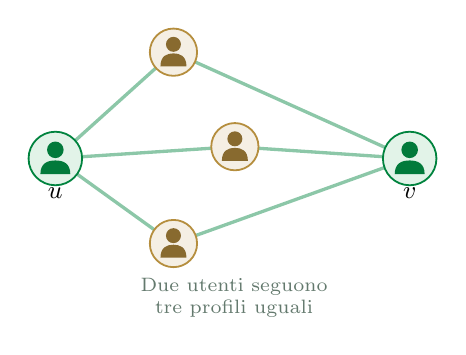
\begin{tikzpicture}[x=1cm,y=1cm]
  \coordinate (u) at (1.05,2.30); \coordinate (v) at (5.55,2.30);
  \coordinate (a) at (2.55,3.65); \coordinate (b) at (3.33,2.45);
  \coordinate (c) at (2.55,1.22);
  \foreach \n in {a,b,c}{\draw[teal!45,line width=1.2pt](u)--(\n);\draw[teal!45,line width=1.2pt](v)--(\n);}
  \pic at (u) {persona}; \pic at (v) {persona};
  \foreach \n in {a,b,c}{\pic at (\n) {contatto};}
  \node[font=\small\bfseries,below=7pt] at (u) {$u$};
  \node[font=\small\bfseries,below=7pt] at (v) {$v$};
  \node[font=\scriptsize,text=muted,align=center] at (3.32,.53)
    {Due utenti seguono\\tre profili uguali};
\end{tikzpicture}
\column{.47\textwidth}
\centering\small\bfseries Articoli: bibliografia in comune
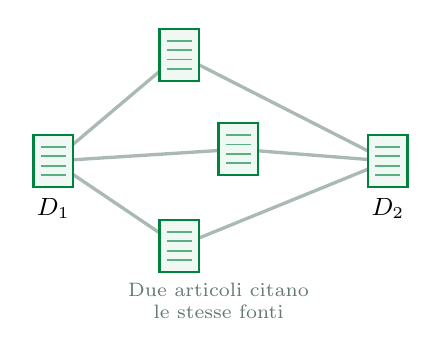
\begin{tikzpicture}[x=1cm,y=1cm]
  \coordinate (p) at (.95,2.30); \coordinate (q) at (5.20,2.30);
  \coordinate (r1) at (2.55,3.65); \coordinate (r2) at (3.30,2.45);
  \coordinate (r3) at (2.55,1.22);
  \foreach \n in {r1,r2,r3}{\draw[ink!36,line width=1.2pt](p)--(\n);\draw[ink!36,line width=1.2pt](q)--(\n);}
  \foreach \n in {p,q,r1,r2,r3}{\pic at (\n) {documento};}
  \node[font=\small\bfseries,below=10pt] at (p) {$D_1$};
  \node[font=\small\bfseries,below=10pt] at (q) {$D_2$};
  \node[font=\scriptsize,text=muted,align=center] at (3.05,.53)
    {Due articoli citano\\le stesse fonti};
\end{tikzpicture}
\end{columns}
\vspace{-.12cm}
\centering\chip{Il vicinato è l'insieme dei profili seguiti o degli articoli citati.}
\end{frame}

% 03 — Tripla originale Input / Query / Goal e confronto grafico
\begin{frame}[t]{Neighborhood Search statico: intersezione e Jaccard}
\vspace{-.16cm}
% La tripla e' fissa: rimane leggibile in tutti e quattro gli overlay.
\begin{columns}[T,onlytextwidth]
  \column{.73\textwidth}
  {\small
  \begin{itemize}
    \item \textbf{Input:} $G=(V,E)$, $\tau\in[0,1]$ e $\sigma:2^V\times2^V\to[0,1]$.\qquad
    \item \textbf{Query:} $S\subseteq V$.\\[4pt]
    \item \textbf{Goal:} trovare $u\in V$ tale che $\sigma(S,N(u))\geq\tau$.
  \end{itemize}
  \par}
  \column{.26\textwidth}
  \centering
  \begin{overlayarea}{\linewidth}{.70cm}
    \centering
    \only<3>{\chip{$\sigma=\text{intersezione}$}}
    \only<4>{\chip{$\sigma=\text{Jaccard}$}\\[2pt]$J(X,Y)=\frac{|X\cap Y|}{|X\cup Y|}$}
  \end{overlayarea}
\end{columns}
\vspace{.20cm}
% 1: La sola tripla. 2: Figure. 3: Intersezioni. 4: Jaccard.
\only<2->{%
  \begin{columns}[T,onlytextwidth]
  \column{.49\textwidth}
  \centering\small\bfseries Insiemi grandi, sovrapposizione minima
  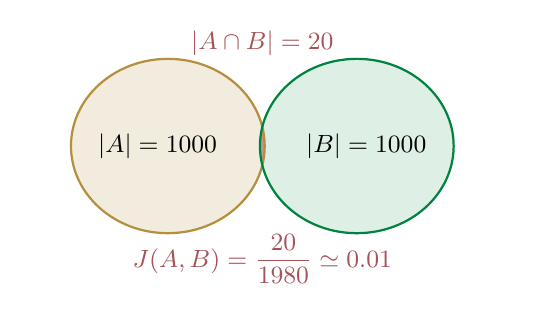
\begin{tikzpicture}[x=1cm,y=.90cm]
    \path[use as bounding box] (.10,-.05) rectangle (6.3,3.70);
    \fill[gold!17] (1.88,2.03) circle (1.23);
    \fill[teal!13] (4.28,2.03) circle (1.23);
    \begin{scope}\clip (1.88,2.03) circle (1.23);
      \fill[coral!68] (4.28,2.03) circle (1.23);
    \end{scope}
    \draw[gold,thick] (1.88,2.03) circle (1.23);
    \draw[teal,thick] (4.28,2.03) circle (1.23);
    \node[font=\small] at (1.75,2.03) {$|A|=1000$};
    \node[font=\small] at (4.40,2.03) {$|B|=1000$};
    \visible<3->{\node[font=\small\bfseries,text=coral!90!black]
      at (3.08,3.48) {$|A\cap B|=20$};}
    \visible<4>{\node[font=\small\bfseries,text=coral!90!black]
      at (3.08,.43) {$J(A,B)=\dfrac{20}{1980}\simeq0.01$};}
  \end{tikzpicture}
  \column{.49\textwidth}
  \centering\small\bfseries Insiemi piccoli, sovrapposizione elevata
   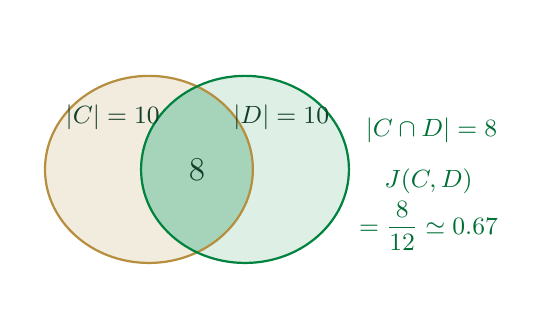
\begin{tikzpicture}[x=1cm,y=.90cm]
    \path[use as bounding box] (.10,-.05) rectangle (6.3,3.70);
    % Totali sempre visibili DENTRO i rispettivi cerchi.
    % Cardinalita' dell'intersezione rivelata all'overlay successivo.
    \fill[gold!17] (1.64,1.70) circle (1.32);
    \fill[teal!13] (2.86,1.70) circle (1.32);
    \begin{scope}\clip (1.64,1.70) circle (1.32);
      \fill[teal!35] (2.86,1.70) circle (1.32);
    \end{scope}
    \draw[gold,thick] (1.64,1.70) circle (1.32);
    \draw[teal,thick] (2.86,1.70) circle (1.32);
    \node[font=\small\bfseries,text=ink] at (1.18,2.44) {$|C|=10$};
    \node[font=\small\bfseries,text=ink] at (3.32,2.44) {$|D|=10$};
    \visible<3->{
      % \node[font=\normalsize\bfseries] at (.95,1.70) {$2$};
      % \node[font=\normalsize\bfseries] at (3.54,1.70) {$2$};
      \node[font=\large\bfseries,text=ink] at (2.25,1.70) {$8$};
      \node[font=\small\bfseries,text=teal!85!black,anchor=west]
        at (4.27,2.25) {$|C\cap D|=8$};
    }
    \visible<4>{\node[font=\small\bfseries,text=teal!85!black,align=center]
      at (5.19,1.13) {$J(C,D)$\\[2pt]$\displaystyle=\frac{8}{12}\simeq0.67$};}
  \end{tikzpicture}
  \end{columns}
  \vspace{-.11cm}
  \begin{overlayarea}{\linewidth}{.82cm}
    \centering
    \only<2>{\chip{Quale coppia di insiemi risulta piu' simile?}}
    \only<3>{\chip{$20>8$: l'intersezione premia gli insiemi grandi,
      senza normalizzare per la loro dimensione.}}
    \only<4>{\chip{$J(A,B)\simeq0.01<0.67\simeq J(C,D)$:
      Jaccard riconosce la maggiore somiglianza relativa.}}
  \end{overlayarea}
}
\end{frame} 

% 04 — LSH introduttiva, senza dettagli di bande
\begin{frame}[t]{Neighborhood Search statico: filter \& verify}
% \vspace{.05cm}
% {\small Data la query $S$, cerchiamo un vertice $u$ con $\sigma(S,N(u))\geq\tau$.\par}
\vspace{.24cm}
\centering{\color{teal}\large\bfseries Soluzione \emph{filter \& verify}}\par
\vspace{.23cm}
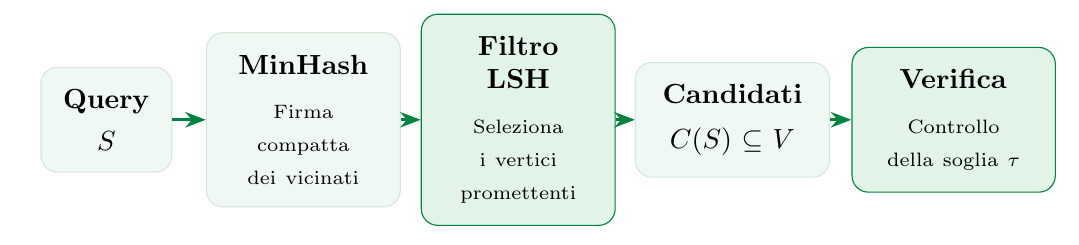
\begin{tikzpicture}[x=1cm,y=1cm]
  \path[use as bounding box] (.0,-.20) rectangle (13.0,2.20);
  \node[block,minimum width=1.15cm,minimum height=.95cm] (query) at (1.00,1.03)
    {\textbf{Query}\\[3pt]$S$};
  \node[block,text width=1.90cm,minimum height=1.15cm] (mh) at (3.50,1.03)
    {\textbf{MinHash}\\[4pt]\scriptsize Firma compatta dei vicinati};
  \node[altblock,text width=1.90cm,minimum height=1.15cm] (lsh) at (6.23,1.03)
    {\textbf{Filtro LSH}\\[4pt]\scriptsize Seleziona i vertici promettenti};
  \node[block,text width=1.90cm,minimum height=1.15cm] (cand) at (8.95,1.03)
    {\textbf{Candidati}\\[4pt]$C(S)\subseteq V$};
  \node[altblock,text width=2.02cm,minimum height=1.15cm] (verify) at (11.76,1.03)
    {\textbf{Verifica}\\[4pt]\scriptsize Controllo della soglia $\tau$};
  \draw[arr] (query.east)--(mh.west);
  \draw[arr] (mh.east)--(lsh.west);
  \draw[arr] (lsh.east)--(cand.west);
  \draw[arr] (cand.east)--(verify.west);
\end{tikzpicture}
\vspace{.12cm}
\begin{columns}[T,onlytextwidth]
\column{.49\textwidth}
\centering\panel{5.55cm}{\textbf{Filter}\\[6pt]\small LSH seleziona i candidati, ma può perdere alcune risposte.}
\column{.49\textwidth}
\centering\panel{5.55cm}{\textbf{Verify}\\[6pt]\small Verifichiamo quali candidati superano la soglia di similarità.}
\end{columns}
\end{frame}

% 05 — Le reti evolvono nel tempo
\begin{frame}[t]{Le reti reali cambiano nel tempo}
\vspace{.22cm}
\begin{columns}[T,onlytextwidth]
\column{.32\textwidth}
\centering\large\bfseries Istante $t_1$\par\vspace{.05cm}
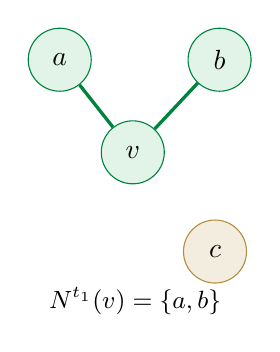
\begin{tikzpicture}[x=.58cm,y=.84cm]
  \node[vert](v)at(2.9,2.7){$v$};\node[vert](a)at(1.3,4.1){$a$};\node[vert](b)at(4.8,4.1){$b$};\node[palevert](c)at(4.7,1.2){$c$};
  \draw[teal,very thick](v)--(a);\draw[teal,very thick](v)--(b);
  \node[font=\small] at (2.95,.45) {$N^{t_1}(v)=\{a,b\}$};
\end{tikzpicture}
\column{.32\textwidth}
\centering\large\bfseries Istante $t_2$\par\vspace{.05cm}
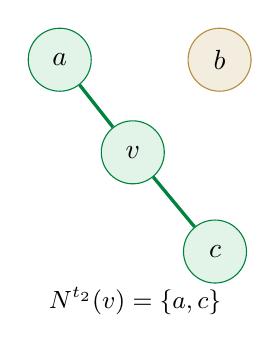
\begin{tikzpicture}[x=.58cm,y=.84cm]
  \node[vert](v)at(2.9,2.7){$v$};\node[vert](a)at(1.3,4.1){$a$};\node[palevert](b)at(4.8,4.1){$b$};\node[vert](c)at(4.7,1.2){$c$};
  \draw[teal,very thick](v)--(a);\draw[teal,very thick](v)--(c);
  \node[font=\small] at (2.95,.45) {$N^{t_2}(v)=\{a,c\}$};
\end{tikzpicture}
\column{.32\textwidth}
\centering\large\bfseries Istante $t_3$\par\vspace{.05cm}
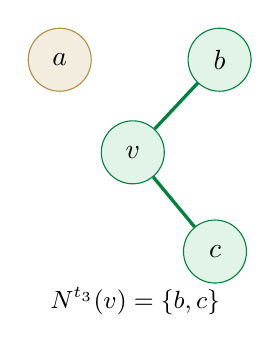
\begin{tikzpicture}[x=.58cm,y=.84cm]
  \node[vert](v)at(2.9,2.7){$v$};\node[palevert](a)at(1.3,4.1){$a$};\node[vert](b)at(4.8,4.1){$b$};\node[vert](c)at(4.7,1.2){$c$};
  \draw[teal,very thick](v)--(b);\draw[teal,very thick](v)--(c);
  \node[font=\small] at (2.95,.45) {$N^{t_3}(v)=\{b,c\}$};
\end{tikzpicture}
\end{columns}
\vspace{.22cm}
\centering\chip{Aggregare tutto in un grafo statico fa perdere l'informazione temporale.}
\end{frame}

% 06 — Grafo temporale a tre nodi
\begin{frame}[t]{Grafo temporale: definizione ed esempio}
\vspace{.08cm}
{\small $\mathcal G=(V,E,\lambda)$: $\lambda(e)$ è l'insieme degli istanti associati all'arco $e$.
Un evento è la tripla $(u,v,t)\in\mathcal E$.\par}
\vspace{.20cm}
\begin{columns}[T,onlytextwidth]
\column{.43\textwidth}
\centering
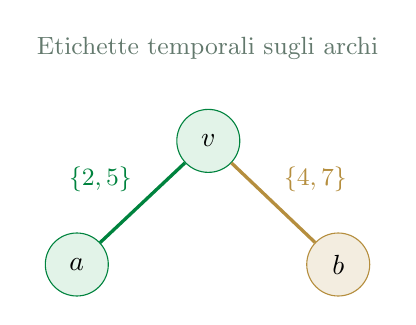
\begin{tikzpicture}[x=1cm,y=1cm]
  \node[vert](v)at(2.35,2.15){$v$};
  \node[vert](a)at(.68,.58){$a$};
  \node[palevert](b)at(4.0,.58){$b$};
  \draw[teal,very thick](v)--node[above left,font=\small]{$\{2,5\}$}(a);
  \draw[gold,very thick](v)--node[above right,font=\small]{$\{4,7\}$}(b);
  \node[font=\small,text=muted] at (2.34,3.33) {Etichette temporali sugli archi};
\end{tikzpicture}
\column{.55\textwidth}
\centering
\panel{6.55cm}{\textbf{Attività del nodo $v$}\\[8pt]
$\Lambda(v)=\{2,4,5,7\}$\\[10pt]
\textbf{Vicinato su un intervallo $I$}\\[8pt]
$\displaystyle N^I(v)=\bigcup_{t\in I}N^t(v)$\\[9pt]
\small $N^{[2,4]}(v)=\{a,b\}$\\[3pt]
\small $N^{[5,6]}(v)=\{a\}$}
\end{columns}
\vspace{-.10cm}
\end{frame}

% 07 — Varianti
\begin{frame}[t]{Due varianti del Neighborhood Search temporale}

\vspace{.03cm}

% La definizione resta sempre visibile.
% Overlay 1: mu appare solo nell'intervallo I.
% Overlay 2: mu >= 0 nell'Input (Variante 1).
% Overlay 3: mu >= 0 nella Query (Variante 2).

\begin{overlayarea}{\textwidth}{1.62cm}
{\small

\textbf{Input:}
$\mathcal G=(V,E,\lambda)$,
$\tau\in[0,1]$
\only<2>{,
$\textcolor{red!80!black}{\boldsymbol{\mu}\geq0}$}.
\\[3pt]

\textbf{Query:}
$S\subseteq V$
\only<3->{e
$\textcolor{red!80!black}{\boldsymbol{\mu}\geq0}$}.
\\[3pt]

\textbf{Goal:}
trovare $u\in V$ e
$I=[t,t+\textcolor{red!80!black}{\boldsymbol{\mu}}]$
tali che
\chip{$J(S,N^I(u))\geq\tau$}.

\par}
\end{overlayarea}

\vspace{.10cm}

\begin{columns}[T,onlytextwidth]

% =====================================================
% VARIANTE 1
% =====================================================

\column{.49\textwidth}
\centering


\begin{tikzpicture}

  \path[use as bounding box]
    (-3.12,-1.53) rectangle (3.12,1.53);

  % Overlay 2: Variante 1 evidenziata
  \only<2>{
    \node[
      draw=teal,
      fill=ice,
      line width=1.7pt,
      rounded corners=9pt,
      minimum width=5.65cm,
      minimum height=2.56cm,
      align=center
    ] at (0,0)
    {
      {\color{teal}\large\bfseries VARIANTE 1}\\[9pt]
      {\Large\bfseries Ampiezza fissa}\\[9pt]
      $\boldsymbol{\mu}$ nell'\textbf{input del problema}
    };
  }

  % Overlay 3: Variante 1 in secondo piano
  \only<3->{
    \node[
      draw=rulegray,
      fill=cloud,
      opacity=.33,
      rounded corners=7pt,
      minimum width=4.3cm,
      minimum height=1.44cm,
      align=center
    ] at (0,0)
    {
      \small\bfseries VARIANTE 1\\[4pt]
      \normalsize Ampiezza fissa
    };
  }

\end{tikzpicture}

% =====================================================
% VARIANTE 2
% =====================================================

\column{.49\textwidth}
\centering


\begin{tikzpicture}

  \path[use as bounding box]
    (-3.12,-1.53) rectangle (3.12,1.53);

  % Overlay 2: Variante 2 in secondo piano
  \only<2>{
    \node[
      draw=rulegray,
      fill=cloud,
      opacity=.33,
      rounded corners=7pt,
      minimum width=4.3cm,
      minimum height=1.44cm,
      align=center
    ] at (0,0)
    {
      \small\bfseries VARIANTE 2\\[4pt]
      \normalsize Ampiezza variabile
    };
  }

  % Overlay 3: Variante 2 evidenziata
  \only<3->{
    \node[
      draw=teal,
      fill=ice,
      line width=1.7pt,
      rounded corners=9pt,
      minimum width=5.65cm,
      minimum height=2.56cm,
      align=center
    ] at (0,0)
    {
      {\color{teal}\large\bfseries VARIANTE 2}\\[9pt]
      {\Large\bfseries Ampiezza variabile}\\[9pt]
      $\boldsymbol{\mu}$ fornita con la \textbf{query}
    };
  }

\end{tikzpicture}
\end{columns}
\end{frame}

\sectslide{01}{Contributi della tesi}{LSH unificato, oracolo $\mathcal O$, pruning temporale\\e rappresentazione geometrica}

% 08 — Contributi variante 1, alto livello
\begin{frame}[t]{Contributo 1: LSH su intervalli di ampiezza fissa}
\vspace{.12cm}
\begin{columns}[T,onlytextwidth]
\column{.52\textwidth}
\begin{itemize}\setlength\itemsep{13pt}
  \item \textbf{Adattamento di LSH} alle coppie nodo--finestra.
  \item \textbf{Pruning $W(v)$} delle finestre inattive.
  \item \textbf{Oracolo $\mathcal O$} per recuperare sketch senza ricostruire vicinati.
  \item \textbf{Analisi teorica} e confronto sperimentale sui grafi reali.
\end{itemize}
\column{.45\textwidth}
\centering
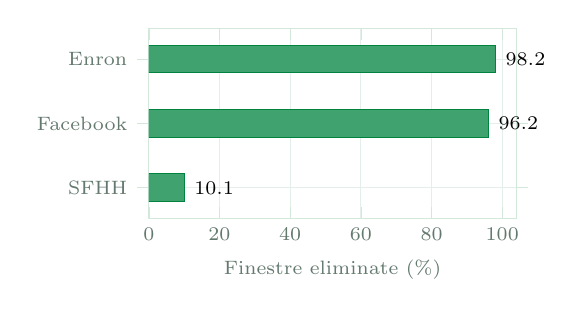
\begin{tikzpicture}
\begin{axis}[xbar,width=6.25cm,height=4.0cm,xmin=0,xmax=104,grid=major,
  symbolic y coords={SFHH,Facebook,Enron},ytick=data,
  xlabel={Finestre eliminate (\%)},nodes near coords,
  every node near coord/.append style={font=\scriptsize},enlarge y limits=.24]
  \addplot[fill=teal!75,draw=teal] coordinates {(10.1,SFHH) (96.2,Facebook) (98.2,Enron)};
\end{axis}
\end{tikzpicture}
\smallnote{Esempio sperimentale: pruning molto diverso tra dataset.}
\end{columns}
\end{frame}

% 09 — Contributi variante 2 e inclusione corretta
\begin{frame}[t]{Contributo 2: un filtro per ampiezze variabili}
\vspace{.06cm}
\begin{columns}[T,onlytextwidth]
\column{.50\textwidth}
\begin{itemize}\setlength\itemsep{13pt}
  \item Indicizzare ogni ampiezza richiederebbe $\Theta(T^2)$ intervalli per nodo.
  \item \textbf{Euristica}: usare la prima componente MinHash per generare candidati.
  \item Rappresentazione geometrica, senza enumerare tutte le finestre.
  \item Nessun bound non banale sul numero di candidati, ma \textbf{pochi in pratica}.
\end{itemize}
\column{.48\textwidth}
\centering
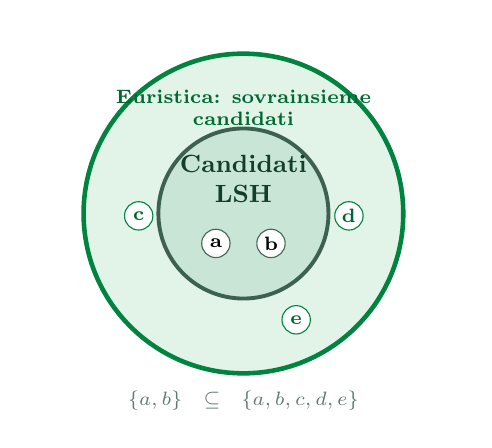
\begin{tikzpicture}[x=1cm,y=1cm]
  \path[use as bounding box](.32,-.36)rectangle(5.86,4.62);
  % Overlay 1: candidati LSH. Overlay 2: compare il sovrainsieme.
  \visible<2->{
    \fill[ice] (3.06,2.26) circle (2.03cm);
    \draw[teal,line width=1.65pt] (3.06,2.26) circle (2.03cm);
    \node[font=\scriptsize\bfseries,text=teal!80!black,align=center] at (3.06,3.60)
      {Euristica: sovrainsieme\\candidati};
  }
  \fill[teal!21] (3.06,2.26) circle (1.08cm);
  \draw[ink!82,line width=1.4pt] (3.06,2.26) circle (1.08cm);
  \node[font=\small\bfseries,text=ink,align=center] at (3.06,2.70)
    {Candidati\\LSH};
  % a,b: candidati della prima banda; c,d,e: ulteriori candidati dell'oracolo.
  \foreach \x/\y/\nm in {2.71/1.88/a,3.41/1.88/b}{
    \node[circle,draw=ink!80,fill=white,minimum size=.36cm,inner sep=0,
      font=\scriptsize\bfseries] at (\x,\y) {\nm};}
  \visible<2->{
    \foreach \x/\y/\nm in {1.73/2.23/c,4.40/2.23/d,3.73/.91/e}{
      \node[circle,draw=teal,fill=white,minimum size=.36cm,inner sep=0,
        font=\scriptsize\bfseries,text=teal!80!black] at (\x,\y) {\nm};}
    \node[font=\scriptsize,text=muted,align=center,text width=5.5cm] at (3.06,-.12)
      {$\{a,b\}\subseteq\{a,b,c,d,e\}$};
  }
\end{tikzpicture}
\end{columns}
\end{frame}

% 10 — Separatore: dettaglio tecnico solo variante 1
\sectslide{02}{Variante 1: soluzione tecnica}{LSH unificato, oracolo $\mathcal O$ e pruning temporale}

% 11 — LSH dettagliato: costruzione e, solo alla fine, probabilità a S
\begin{frame}[t]{LSH nel dettaglio: bande e tabelle hash}
\vspace{.04cm}
{\small Lo sketch MinHash contiene $k=br$ valori; ogni \textbf{banda} (di $r$ righe) va in una delle $b$ tabelle hash.}
\vspace{.05cm}
\centering
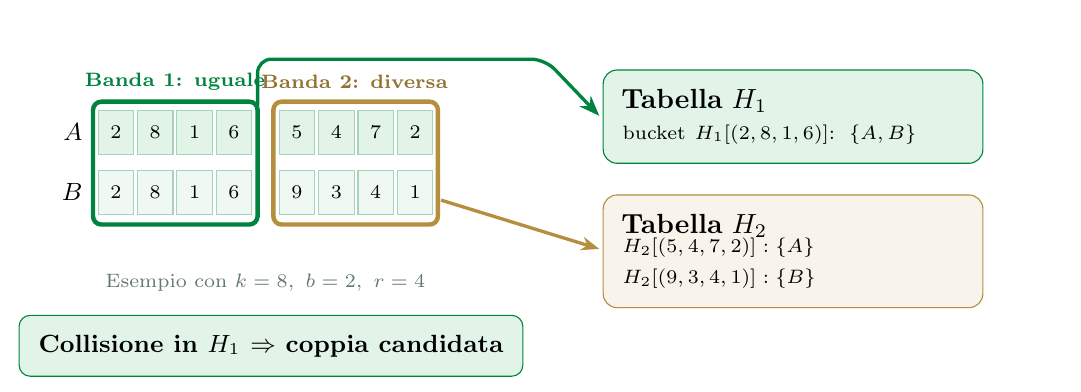
\begin{tikzpicture}[x=1cm,y=1cm]
  \path[use as bounding box] (.08,.25) rectangle (13.1,4.52);
  \node[font=\scriptsize,text=muted] at (3.10,1.28) {Esempio con $k=8,\ b=2,\ r=4$};
  \node[font=\small\bfseries,anchor=east] at (.90,3.19) {$A$};
  \node[font=\small\bfseries,anchor=east] at (.90,2.43) {$B$};
  \foreach \val/\x in {2/1.20,8/1.70,1/2.20,6/2.70,5/3.50,4/4.00,7/4.50,2/5.00}
    {\node[draw=teal!35,fill=ice,minimum width=.45cm,minimum height=.56cm,font=\scriptsize] at (\x,3.19) {\val};}
  \foreach \val/\x in {2/1.20,8/1.70,1/2.20,6/2.70,9/3.50,3/4.00,4/4.50,1/5.00}
    {\node[draw=teal!35,fill=cloud,minimum width=.45cm,minimum height=.56cm,font=\scriptsize] at (\x,2.43) {\val};}
  \draw[teal,line width=1.6pt,rounded corners=3pt](.91,2.02)rectangle(3.00,3.58);
  \draw[gold,line width=1.6pt,rounded corners=3pt](3.20,2.02)rectangle(5.29,3.58);
  \node[font=\scriptsize\bfseries,text=teal] at (1.95,3.83) {Banda 1: uguale};
  \node[font=\scriptsize\bfseries,text=gold!80!black] at (4.23,3.83) {Banda 2: diversa};
  \visible<2-3>{
    \draw[arr,rounded corners=5pt] (3.00,3.53) -- (3.00,4.12) -- (6.65,4.12) -- (7.34,3.40);
    \draw[-{Stealth[length=2.3mm]},line width=1.2pt,draw=gold] (5.33,2.33) -- (7.34,1.71);
    \node[draw=teal,fill=ice,rounded corners=5pt,text width=4.33cm,align=left,inner sep=7pt] at (9.80,3.39)
      {\textbf{Tabella $H_1$}\\[-1pt]\scriptsize bucket $H_1[(2,8,1,6)]$: $\{A,B\}$};
    \node[draw=gold,fill=gold!10,rounded corners=5pt,text width=4.33cm,align=left,inner sep=7pt] at (9.80,1.68)
      {\textbf{Tabella $H_2$}\\[-1pt]\scriptsize $H_2[(5,4,7,2)]:\{A\}$\\[-1pt]
       \scriptsize $H_2[(9,3,4,1)]:\{B\}$};
  }
  \visible<3>{
    \node[draw=teal,fill=ice,rounded corners=4pt,inner sep=7pt,font=\small\bfseries]
      at (3.17,.48) {Collisione in $H_1$ $\Rightarrow$ coppia candidata};
  }
\end{tikzpicture}
\end{frame}

% 12 — Adattamento LSH
\begin{frame}[t]{Adattamento temporale: $b$ tabelle condivise e doppia chiave}
\vspace{.06cm}
\centering
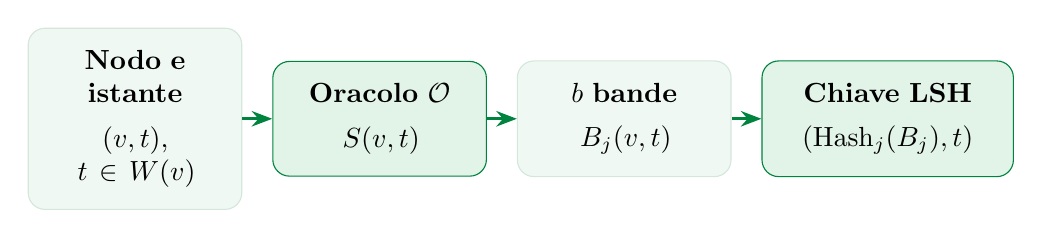
\begin{tikzpicture}[node distance=.38cm]
  \node[block,text width=2.15cm,minimum height=1.17cm](a){\textbf{Nodo e istante}\\[4pt]$(v,t)$, $t\in W(v)$};
  \node[altblock,right=of a,text width=2.15cm,minimum height=1.17cm](b){\textbf{Oracolo $\mathcal O$}\\[4pt]$S(v,t)$};
  \node[block,right=of b,text width=2.15cm,minimum height=1.17cm](c){\textbf{$b$ bande}\\[4pt]$B_j(v,t)$};
  \node[altblock,right=of c,text width=2.63cm,minimum height=1.17cm](d){\textbf{Chiave LSH}\\[4pt]$(\operatorname{Hash}_j(B_j),t)$};
  \draw[arr](a)--(b);\draw[arr](b)--(c);\draw[arr](c)--(d);
\end{tikzpicture}
\vspace{.17cm}
\begin{center}
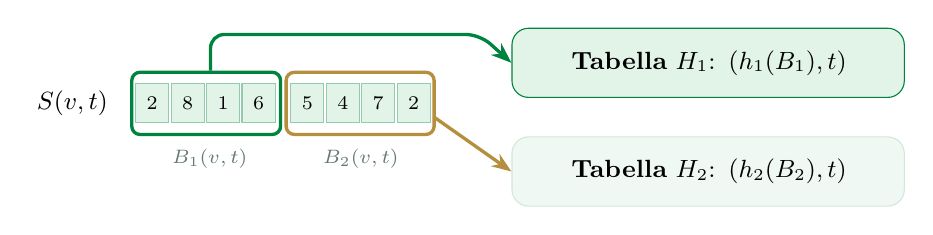
\begin{tikzpicture}[x=1cm,y=1cm]
  \node[font=\small\bfseries,anchor=east] at (1.83,1.35) {$S(v,t)$};
  \foreach \val/\x in {2/2.27,8/2.72,1/3.17,6/3.62,5/4.24,4/4.69,7/5.14,2/5.59}
    {\node[draw=teal!42,fill=ice,minimum width=.42cm,minimum height=.50cm,font=\scriptsize]at(\x,1.35){\val};}
  \draw[teal,very thick,rounded corners=3pt](2.01,.95)rectangle(3.90,1.74);
  \draw[gold,very thick,rounded corners=3pt](3.97,.95)rectangle(5.85,1.74);
  \node[font=\scriptsize,text=muted]at(3.0,.64){$B_1(v,t)$};
  \node[font=\scriptsize,text=muted]at(4.92,.64){$B_2(v,t)$};
  \node[altblock,text width=4.42cm,font=\small] (H1) at (9.33,1.86)
    {\textbf{Tabella $H_1$}: $(h_1(B_1),t)$};
  \node[block,text width=4.42cm,font=\small] (H2) at (9.33,.48)
    {\textbf{Tabella $H_2$}: $(h_2(B_2),t)$};
  \draw[arr,rounded corners=5pt](3.01,1.76)--(3.01,2.22)--(6.43,2.22)--(H1.west);
  \draw[-{Stealth[length=2.5mm]},draw=gold,line width=1.2pt](5.85,1.17)--(H2.west);
\end{tikzpicture}
\end{center}
\vspace{-.04cm}
\begin{columns}[T,onlytextwidth]
\column{.49\textwidth}\centering{\small\bfseries Uniche $b$ tabelle per ogni $\mu$ fissata}\\
\smallnote{Tutti i nodi e gli inizi di finestra condividono le tabelle.}
\column{.49\textwidth}\centering{\small\bfseries Timestamp incluso nella chiave}\\
\smallnote{Firme uguali in finestre diverse finiscono in bucket differenti.}
\end{columns}
\vspace{.01cm}
\end{frame}

% 13 — Pruning e caso pessimo: attenzione, nessun miglioramento asintotico
\begin{frame}[t]{Pruning $W(v)$: meno finestre, stesso caso peggiore}
\vspace{.01cm}
\centering\chip{$W(v)=\{t:\ [t,t+\mu]\cap\Lambda(v)\neq\varnothing\}$}\par
\vspace{.10cm}
{\small\textbf{Esempio:} $T=12$, $\mu=2$, $\Lambda(v)=\{4,9\}$.
Una finestra si conserva soltanto se contiene un evento di $v$.\par}
\vspace{.08cm}
\centering
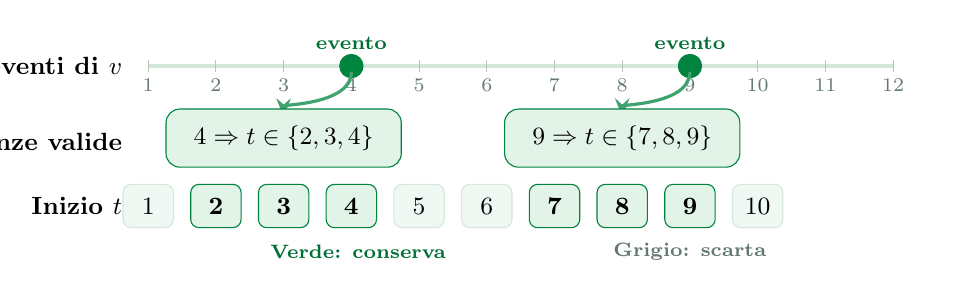
\begin{tikzpicture}[x=.86cm,y=.75cm]
  \path[use as bounding box] (.22,.06) rectangle (13.80,4.13);

  % Riga 1: sulla linea temporale evidenziamo soltanto i due eventi.
  \node[font=\small\bfseries,anchor=east] at (1.76,3.48) {Eventi di $v$};
  \draw[rulegray,line width=1.5pt] (2,3.48)--(13,3.48);
  \foreach \t in {1,...,12}{
    \pgfmathsetmacro{\xx}{\t+1}
    \draw[muted!45] (\xx,3.38)--(\xx,3.58);
    \node[font=\scriptsize,text=muted] at (\xx,3.16) {\t};
  }
  \foreach \t in {4,9}{
    \pgfmathsetmacro{\xx}{\t+1}
    \fill[teal] (\xx,3.48) circle (4.4pt);
    \node[font=\scriptsize\bfseries,text=teal!85!black] at (\xx,3.86) {evento};
  }

  % Riga 2: un evento a s rende valide le partenze da s-mu a s.
  \node[font=\small\bfseries,anchor=east] at (1.76,2.20) {Partenze valide};
  \draw[-{Stealth[length=2.4mm]},teal!75,line width=1.15pt]
    (5,3.38) .. controls (5,2.83) and (4,2.83) .. (4,2.61);
  \draw[-{Stealth[length=2.4mm]},teal!75,line width=1.15pt]
    (10,3.38) .. controls (10,2.83) and (9,2.83) .. (9,2.61);
  \node[draw=teal,fill=ice,rounded corners=5pt,inner xsep=10pt,inner ysep=6pt,
    font=\small\bfseries] at (4,2.26) {$4\Rightarrow t\in\{2,3,4\}$};
  \node[draw=teal,fill=ice,rounded corners=5pt,inner xsep=10pt,inner ysep=6pt,
    font=\small\bfseries] at (9,2.26) {$9\Rightarrow t\in\{7,8,9\}$};

  % Riga 3: tutti i possibili inizi di finestra; verdi quelli da conservare.
  \node[font=\small\bfseries,anchor=east] at (1.76,1.11) {Inizio $t$};
  \foreach \t in {1,5,6,10}{
    \pgfmathsetmacro{\xx}{\t+1}
    \node[draw=rulegray,fill=cloud,rounded corners=3pt,
      minimum width=.64cm,minimum height=.55cm,font=\small]
      at (\xx,1.11) {\t};
  }
  \foreach \t in {2,3,4,7,8,9}{
    \pgfmathsetmacro{\xx}{\t+1}
    \node[draw=teal,fill=ice,rounded corners=3pt,
      minimum width=.64cm,minimum height=.55cm,font=\small\bfseries]
      at (\xx,1.11) {\t};
  }
  \node[font=\scriptsize\bfseries,text=teal!85!black] at (5.10,.34)
    {Verde: conserva};
  \node[font=\scriptsize\bfseries,text=muted] at (10.00,.34)
    {Grigio: scarta};
\end{tikzpicture}
\vspace{-.07cm}
\centering\chip{$10$ finestre possibili $\;\longrightarrow\;$ $|W(v)|=6$: $4$ finestre scartate}\par
\vspace{.35cm}
{\small $\displaystyle |W(v)|\leq\min\{T-\mu,(\mu+1)|\Lambda(v)|\}$}\par
\vspace{.08cm}
\smallnote{\textbf{Caso peggiore invariato}: se ogni finestra contiene un evento, $|W(v)|=T-\mu$. Il pruning è utile se l'attività è temporalmente sparsa.}
\end{frame}

% 14 — Bound teorici recuperati dalla prima presentazione
\begin{frame}[t]{Bound teorici ottenuti}
\vspace{.10cm}
\begin{center}\small $w_v=|W(v)|$, $m_v=|\Lambda(v)|$ e $C_v=\sum_{t\in W(v)}|C(v,t)|$ candidati esaminati.\end{center}
\vspace{.24cm}
\begin{columns}[T,onlytextwidth]
\column{.33\textwidth}\centering
\panel{4.02cm}{\textbf{Costruzione indice}\\[12pt]
$\displaystyle O\!\left(\sum_{v\in V}w_v(k\log m_v+b)\right)$\\[10pt]
\scriptsize Preprocessing delle $b$ tabelle}
\column{.33\textwidth}\centering
\panel{4.02cm}{\textbf{Spazio indice}\\[12pt]
$\displaystyle O\!\left(b\sum_{v\in V}w_v\right)$\\[10pt]
\scriptsize Bucket delle finestre indicizzate}
\column{.33\textwidth}\centering
\panel{4.02cm}{\textbf{Tempo di query}\\[12pt]
$\displaystyle O\!\left(w_v(k\log m_v+b)+kC_v\right)$\\[10pt]
\scriptsize Inclusa la verifica delle firme}
\end{columns}
\vspace{.13cm}
\vspace{.07cm}
% \begin{center}\begin{minipage}{12.2cm}\centering
% \smallnote{Nel caso peggiore $w_v=T-\mu$: nessun miglioramento asintotico. I bound riguardano l'indice LSH; costruzione e memoria dell'oracolo $\mathcal O$ si contabilizzano separatamente.}
% \end{minipage}\end{center}
\end{frame}

% 14 — Valutazione di W sui dataset reali
\begin{frame}[t]{Il pruning nei dataset reali}
\vspace{.04cm}
\centering\small\bfseries Percentuale media di finestre scartate con $W(v)$, su $T-\mu$ finestre totali
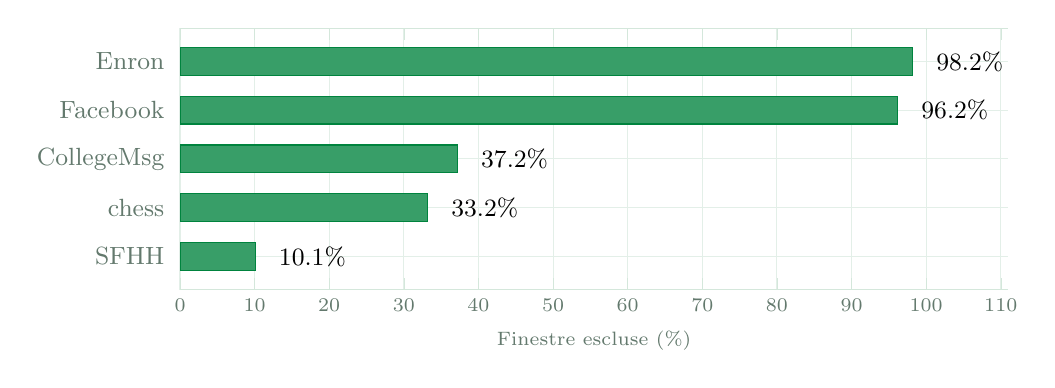
\begin{tikzpicture}
\begin{axis}[xbar,width=12.1cm,height=4.90cm,xmin=0,xmax=111,grid=major,
  symbolic y coords={SFHH,chess,CollegeMsg,Facebook,Enron},ytick=data,
  yticklabel style={font=\small},xlabel={Finestre escluse (\%)},
  axis y line=left,y axis line style={draw=none},ytick style={draw=none},
  nodes near coords,point meta=explicit symbolic,
  every node near coord/.append style={font=\small,anchor=west,xshift=5pt,yshift=0pt},
  enlarge y limits=.17]
  \addplot[fill=teal!78,draw=teal] coordinates {
    (10.1,SFHH) [10.1\%] (33.2,chess) [33.2\%]
    (37.2,CollegeMsg) [37.2\%] (96.2,Facebook) [96.2\%]
    (98.2,Enron) [98.2\%]};
\end{axis}
\end{tikzpicture}
\vspace{-.08cm}
\begin{center}\chip{Enron: $98.2\%$}\qquad\chip{SFHH: $10.1\%$}\end{center}
\smallnote{Attività temporalmente sparsa: pruning molto efficace. Attività diffusa nel tempo: guadagno limitato.}
\end{frame}

% Approfondimento 1 — Grafico originale pruning_analysis su SFHH
% \begin{frame}[t]{Pruning su SFHH-conf-sensor: guadagno limitato}
% \vspace{.03cm}
% \begin{center}
%   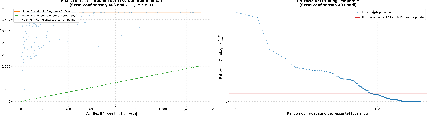
\includegraphics[width=.94\linewidth,height=4.72cm,keepaspectratio]{figures/pruning_sfhh.pdf}
% \end{center}
% \vspace{-.09cm}
% \begin{center}
%   \chip{$10.1\%$ delle finestre eliminate}
%   \qquad\chip{Guadagno medio $1.19\times$}
% \end{center}
% \vspace{-.01cm}
% \smallnote{Con eventi distribuiti su molti istanti temporali, $W(v)$ rimane vicino all'insieme delle finestre ammissibili.}
% \end{frame}

% Approfondimento 2 — Grafico originale pruning_analysis su Enron
\begin{frame}[t]{Pruning su Enron-email: guadagno elevato}
\vspace{.03cm}
\begin{center}
  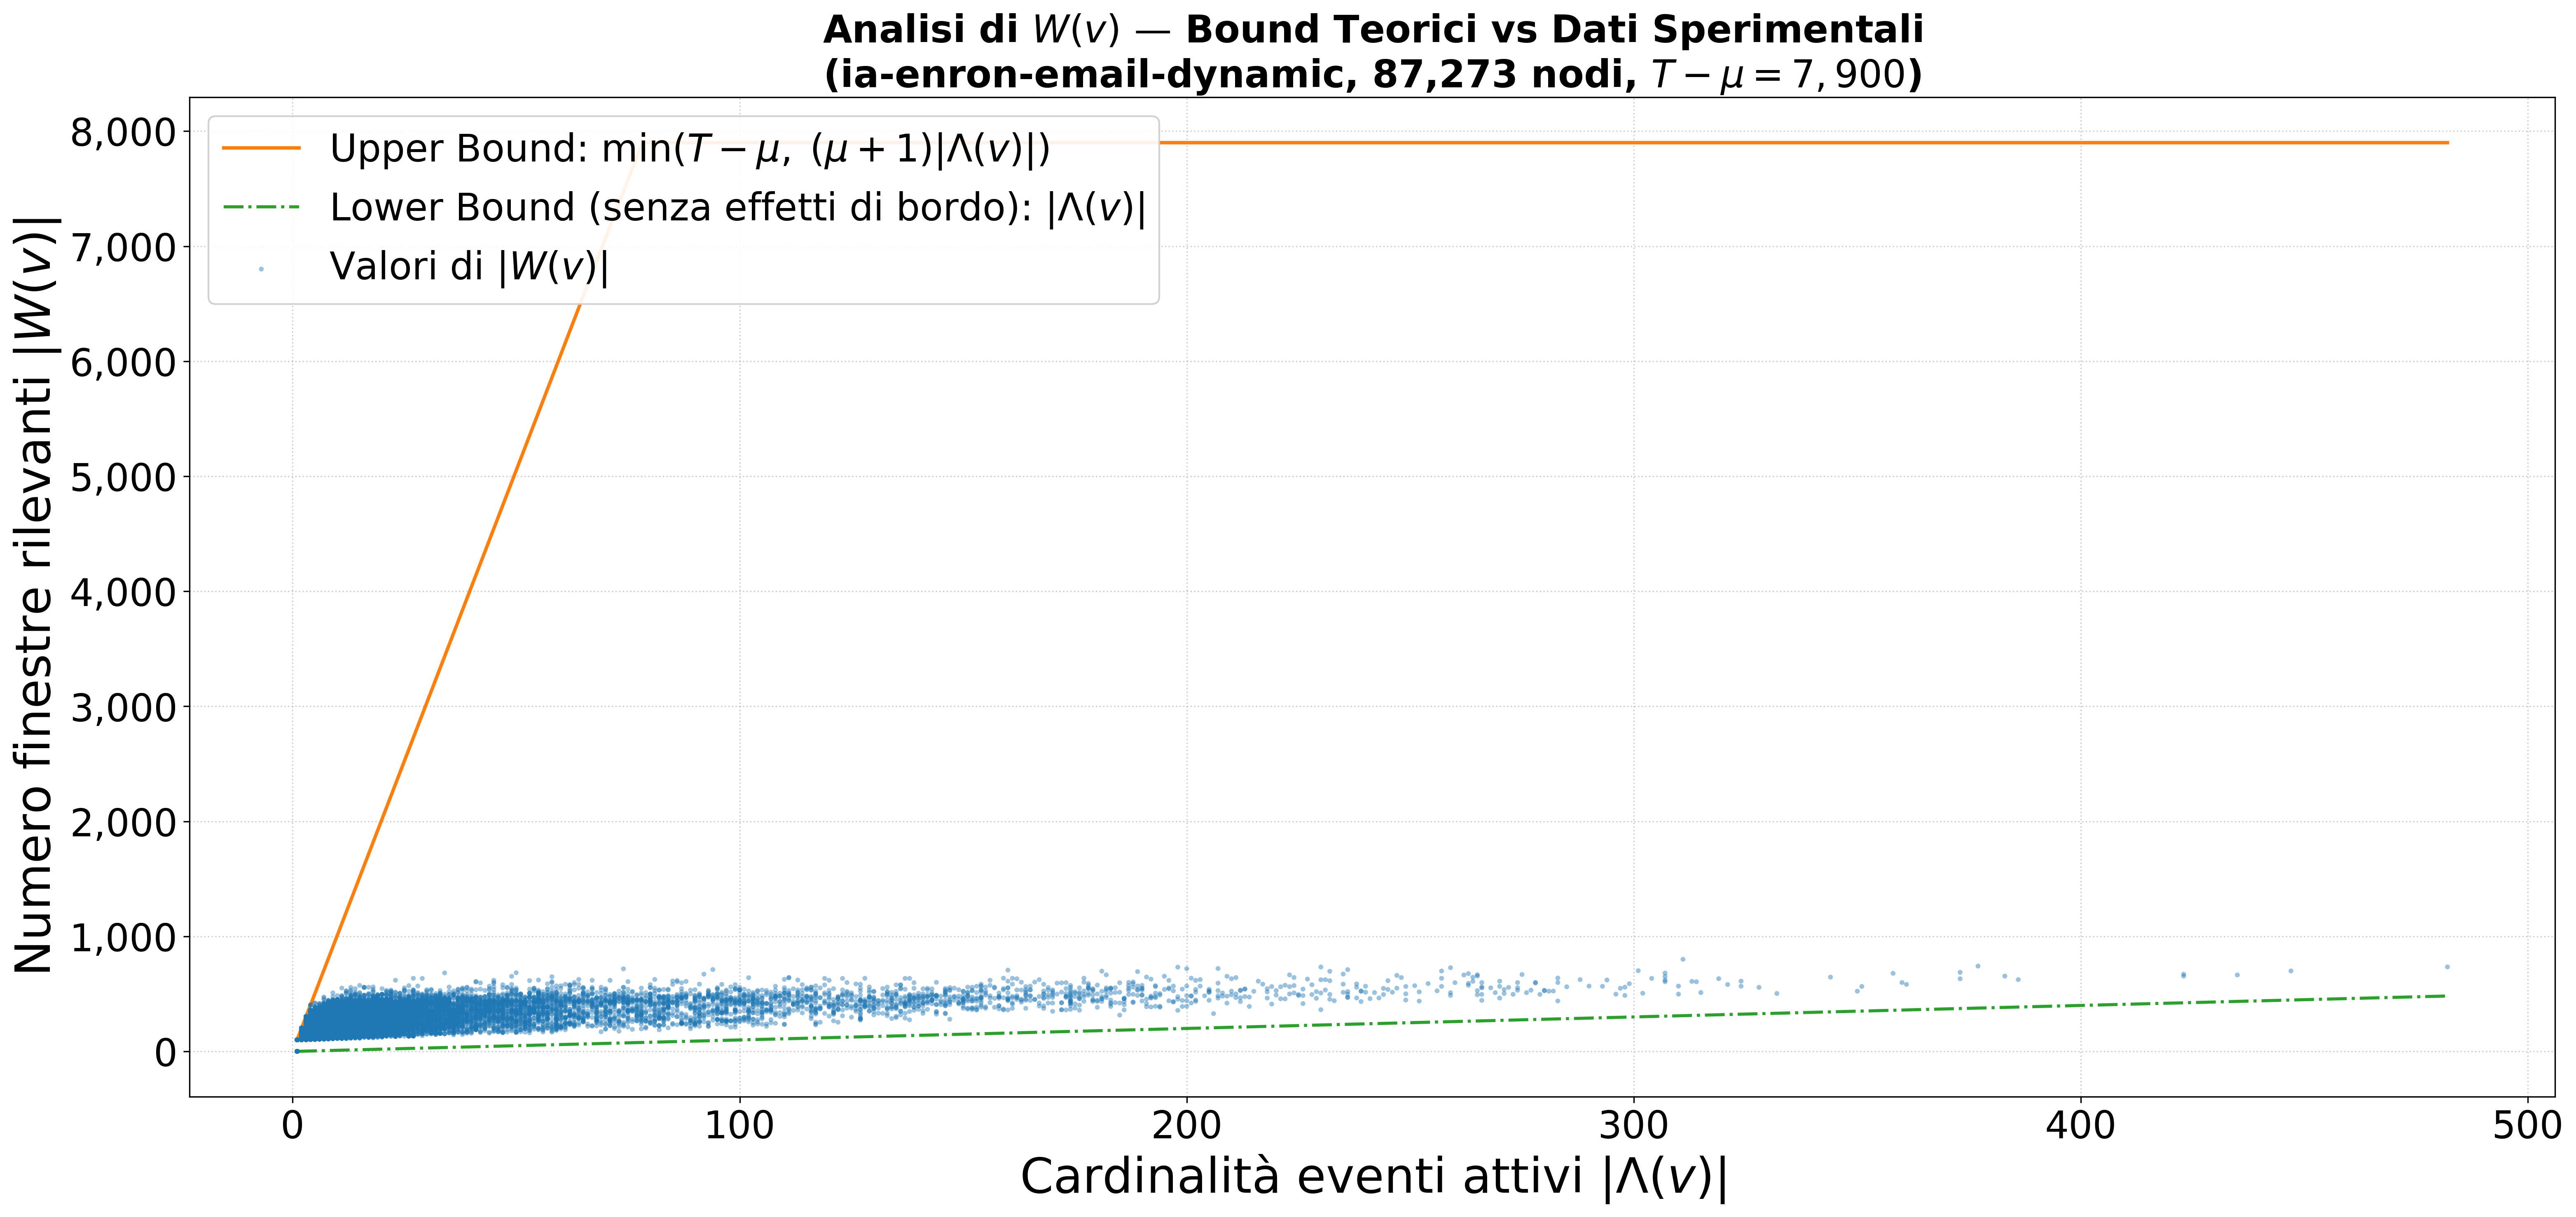
\includegraphics[width=.94\linewidth,height=4.72cm,keepaspectratio]{figures/ia-enron-email-dynamic_pruning_analysis_only_bound.png}
\end{center}
\vspace{-.09cm}
\begin{center}
  \chip{$98.2\%$ delle finestre eliminate}
  \qquad\chip{Da $7900$ a $158$ finestre in media}
\end{center}
\vspace{-.01cm}
\smallnote{La concentrazione degli eventi in pochi istanti consente di escludere molte finestre senza attività.}
\end{frame}

% 15 — Benchmark prestazionale sulle query
% \begin{frame}[t]{Prestazioni: Brute Force contro LSH+$W$}
% \vspace{.01cm}
% \begin{center}\small\bfseries Parametri degli esperimenti: $k=128,\quad b=8,\quad r=16,\quad\tau=0.35$.\end{center}
% \vspace{-.16cm}
% \begin{center}
% 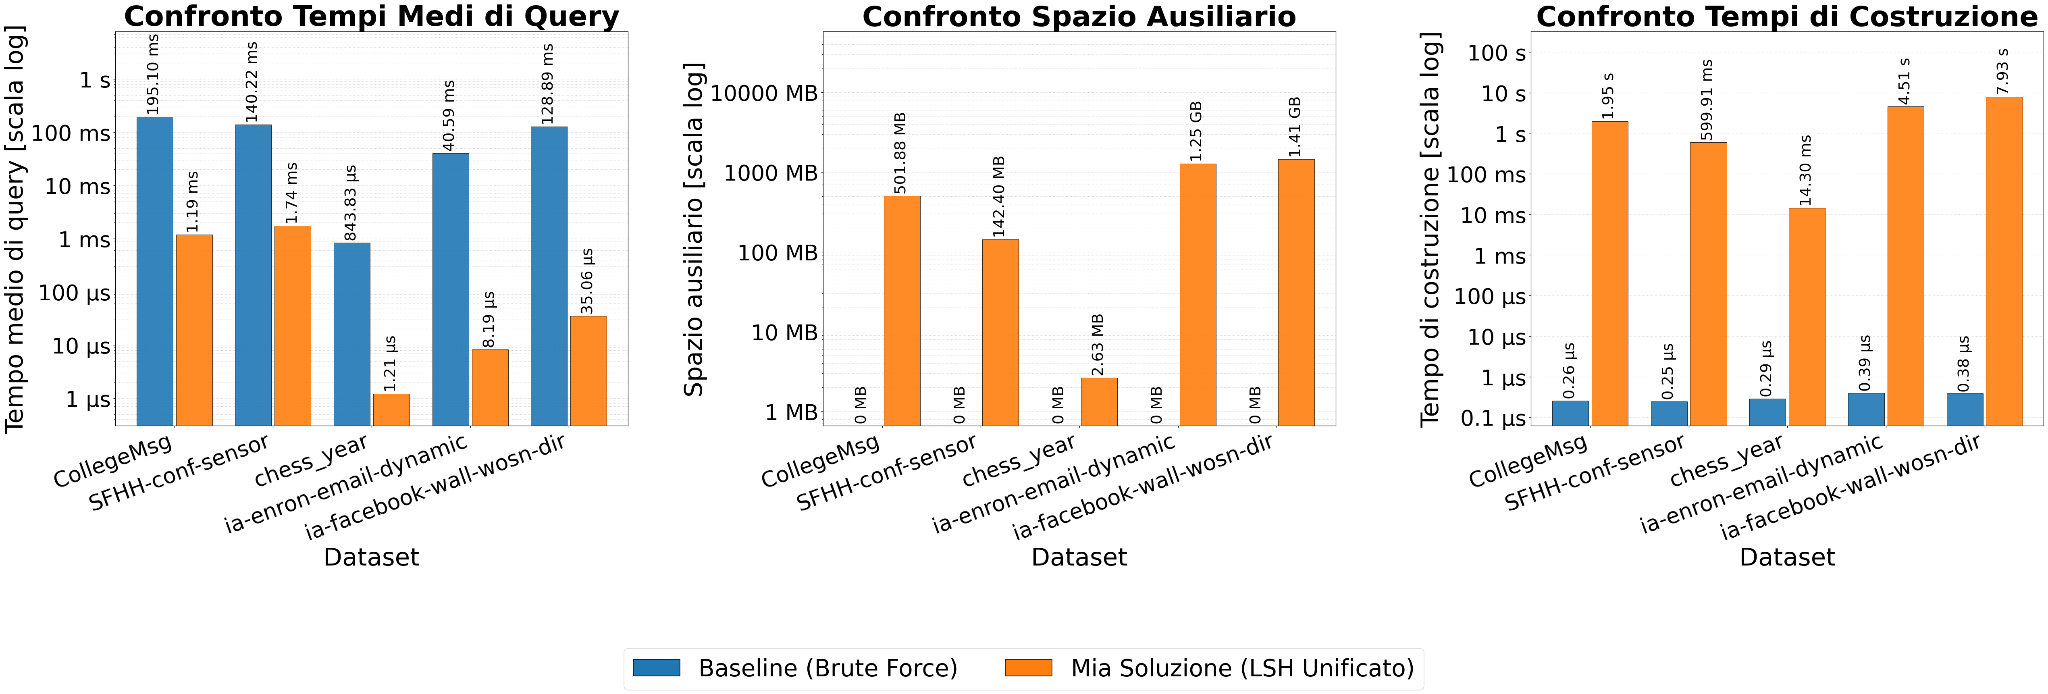
\includegraphics[width=.98\linewidth,height=4.45cm,keepaspectratio]{figures/benchmark_baseline.png}
% \end{center}
% \vspace{-.15cm}
% \begin{center}
% \chip{Enron: $8431\times$ più veloce}\quad\chip{Facebook: $4287\times$ più veloce}
% \end{center}
% \smallnote{Enron: BF $82\,757.90\,\mu$s, LSH+$W$ $9.82\,\mu$s. La query booleana si arresta al primo esito positivo.}
% \end{frame}

% 16 — Confronto con altre strategie
% \begin{frame}[t]{Qual è il contributo del pruning e dell'indice unico?}
% \vspace{.10cm}
% \begin{columns}[T,onlytextwidth]
% \column{.54\textwidth}
% \centering\small\bfseries Tempo medio di query su Enron ($\mu$s)
% \begin{tikzpicture}
% \begin{axis}[ybar,width=7.55cm,height=6.65cm,ymin=0,ymax=112,grid=major,
%   symbolic x coords={NostraSoluzione,Baseline,LSH-W},xtick=data,bar width=22pt,
%   nodes near coords,every node near coord/.append style={font=\small},
%   enlarge x limits=.24]
%   \addplot[fill=teal!77,draw=teal] coordinates {(NostraSoluzione,9.82) (LSH-W,91.88) (Baseline,34.64)};
% \end{axis}
% \end{tikzpicture}
% \column{.43\textwidth}
% \vspace{.36cm}
% \panel{5.1cm}{\textbf{NostraSoluzione}\\[5pt]\small Indice unico con pruning.}
% \vspace{.11cm}
% \panel{5.1cm}{\textbf{Baseline}\\[5pt]\small Indici indipendenti per ogni finestra.}
% \vspace{.11cm}
% \panel{5.1cm}{\textbf{LSH--$W$}\\[5pt]\small Stesso indice, senza pruning.}
% \end{columns}
% \vspace{-.07cm}
% \end{frame}
\begin{frame}[t]{Qual è il contributo del pruning e dell'indice unico?}
\vspace{.10cm}

\begin{columns}[T,onlytextwidth]

\column{.54\textwidth}
\centering\small\bfseries Tempo medio di query su Enron ($\mu$s)

\begin{tikzpicture}

\begin{axis}[
    ybar,
    width=7.55cm,
    height=6.65cm,
    ymin=0,
    ymax=125,
    grid=major,
    symbolic x coords={NostraSoluzione,Baseline,LSH-W},
    xtick=data,
    bar width=22pt,
    enlarge x limits=.24
]

% =========================================================
% BARRE — SEMPRE VISIBILI
% =========================================================

\addplot[
    fill=teal!77,
    draw=teal
] coordinates {
    (NostraSoluzione,9.82)
    (Baseline,34.64)
    (LSH-W,91.88)
};


% =========================================================
% ANIMAZIONE 2 — SPEEDUP VS BASELINE (ROSSO)
% =========================================================

\only<2->{

    \draw[
        red!85!black,
        opacity=.70,
        line width=1.5pt,
        dash pattern=on 4pt off 2.5pt
    ]
        ([xshift=10pt]axis cs:NostraSoluzione,9.82)

        -- ([xshift=16pt]axis cs:NostraSoluzione,9.82)

        -- ([xshift=16pt]axis cs:NostraSoluzione,55)

        -- node[
            midway,
            above=4pt,
            fill=white,
            rounded corners=2pt,
            inner sep=3pt,
            font=\small\bfseries,
            text=red!85!black,
            opacity=1
        ] {$3.5\times$}
        ([xshift=-10pt]axis cs:Baseline,55)

        -- ([xshift=-10pt]axis cs:Baseline,34.64);


    % Punti di contatto rossi
    \fill[red!85!black]
        ([xshift=10pt]axis cs:NostraSoluzione,9.82)
        circle (1.8pt);

    \fill[red!85!black]
        ([xshift=-10pt]axis cs:Baseline,34.64)
        circle (1.8pt);
}


% =========================================================
% ANIMAZIONE 3 — SPEEDUP VS LSH-W (BLU)
% =========================================================

\only<3->{

    \draw[
        blue!80!black,
        opacity=.70,
        line width=1.5pt,
        dash pattern=on 4pt off 2.5pt
    ]
        ([xshift=-10pt]axis cs:NostraSoluzione,9.82)

        -- ([xshift=-16pt]axis cs:NostraSoluzione,9.82)

        -- ([xshift=-16pt]axis cs:NostraSoluzione,108)

        -- node[
            midway,
            above=4pt,
            fill=white,
            rounded corners=2pt,
            inner sep=3pt,
            font=\small\bfseries,
            text=blue!80!black,
            opacity=1
        ] {$9.4\times$}
        ([xshift=-10pt]axis cs:LSH-W,108)

        -- ([xshift=-10pt]axis cs:LSH-W,91.88);


    % Punti di contatto blu
    \fill[blue!80!black]
        ([xshift=-10pt]axis cs:NostraSoluzione,9.82)
        circle (1.8pt);

    \fill[blue!80!black]
        ([xshift=-10pt]axis cs:LSH-W,91.88)
        circle (1.8pt);
}


% =========================================================
% VALORI DELLE BARRE — SEMPRE VISIBILI
% Disegnati per ultimi per garantirne la leggibilità
% =========================================================

\node[
    font=\small,
    fill=white,
    inner sep=1.5pt,
    anchor=south
] at ([yshift=3pt]axis cs:NostraSoluzione,9.82)
    {9.82};

\node[
    font=\small,
    fill=white,
    inner sep=1.5pt,
    anchor=south
] at ([yshift=3pt]axis cs:Baseline,34.64)
    {34.64};

\node[
    font=\small,
    fill=white,
    inner sep=1.5pt,
    anchor=south
] at ([yshift=3pt]axis cs:LSH-W,91.88)
    {91.88};

\end{axis}

\end{tikzpicture}


% =========================================================
% DESCRIZIONE DELLE SOLUZIONI — SEMPRE VISIBILE
% =========================================================

\column{.43\textwidth}

\vspace{.36cm}

\panel{5.1cm}{
    \textbf{NostraSoluzione}\\[5pt]
    \small Indice unico con pruning.
}

\vspace{.11cm}

\panel{5.1cm}{
    \textbf{Baseline}\\[5pt]
    \small Indici indipendenti per ogni finestra.
}

\vspace{.11cm}

\panel{5.1cm}{
    \textbf{LSH--$W$}\\[5pt]
    \small Stesso indice, senza pruning.
}

\end{columns}

\vspace{-.07cm}

\end{frame}

% 17 — Richiesta esplicita: qualità risposte e falsi negativi
\begin{frame}[t]{Il compromesso probabilistico: la recall}
\vspace{.07cm}
\begin{columns}[T,onlytextwidth]
\column{.73\textwidth}
\centering\small\bfseries Recall della soluzione rispetto alla Ground Truth
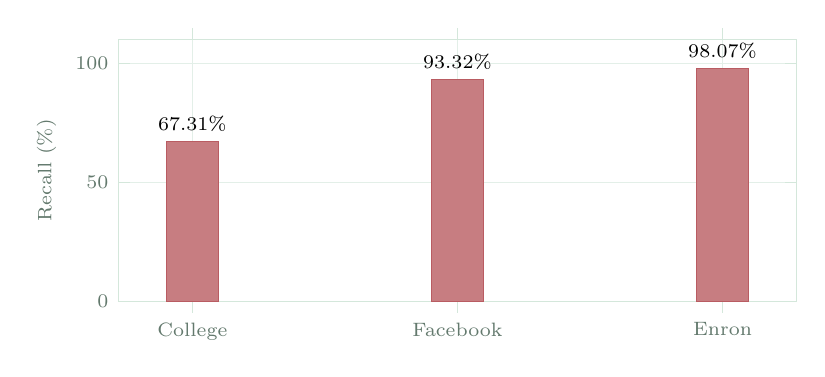
\begin{tikzpicture}
\begin{axis}[ybar,width=10.2cm,height=4.9cm,ymin=0,ymax=110,grid=major,bar width=19pt,
 symbolic x coords={College,Facebook,Enron},xtick=data,
 ylabel={Recall (\%)},enlarge x limits=.14,
 nodes near coords,point meta=explicit symbolic,
 every node near coord/.append style={font=\scriptsize}]
 \addplot[fill=coral!80,draw=coral] coordinates {
   (College,67.31) [67.31\%] (Facebook,93.32) [93.32\%]
   (Enron,98.07) [98.07\%]};
\end{axis}
\end{tikzpicture}
\column{.25\textwidth}
\vspace{.50cm}
\panel{2.8cm}{\textbf{Falsi negativi}\\[7pt]\scriptsize Il filtro può scartare nodi con similarità sufficiente.}
\vspace{.24cm}
% \panel{2.8cm}{\textbf{Recall}\\[7pt]$\displaystyle \frac{|B\cap L|}{|B|}$}
\panel{2.8cm}{\textbf{Dati}\\[5pt]$\displaystyle k=128,b=8,r=16,\tau=0.35$}
\end{columns}
\vspace{.02cm}
\smallnote{Ground Truth calcolata tramite \textbf{Ricerca Esaustiva}, sulle medesime firme MinHash. Zero falsi posiviti}
\end{frame}

% variante 2 spostata dopo le conclusioni per questioni di tempo
% 18 — Separatore variante 2
\sectslide{03}{Variante 2: filtro geometrico}{Una soluzione euristica per ampiezze variabili}
% 21 — Risultati empirici sul numero di candidati: le figure originali dell'esperimento
\begin{frame}[t]{Il filtro euristico restituisce pochi candidati in pratica}
\vspace{.04cm}
\begin{columns}[T,onlytextwidth]
\column{.49\textwidth}
\centering
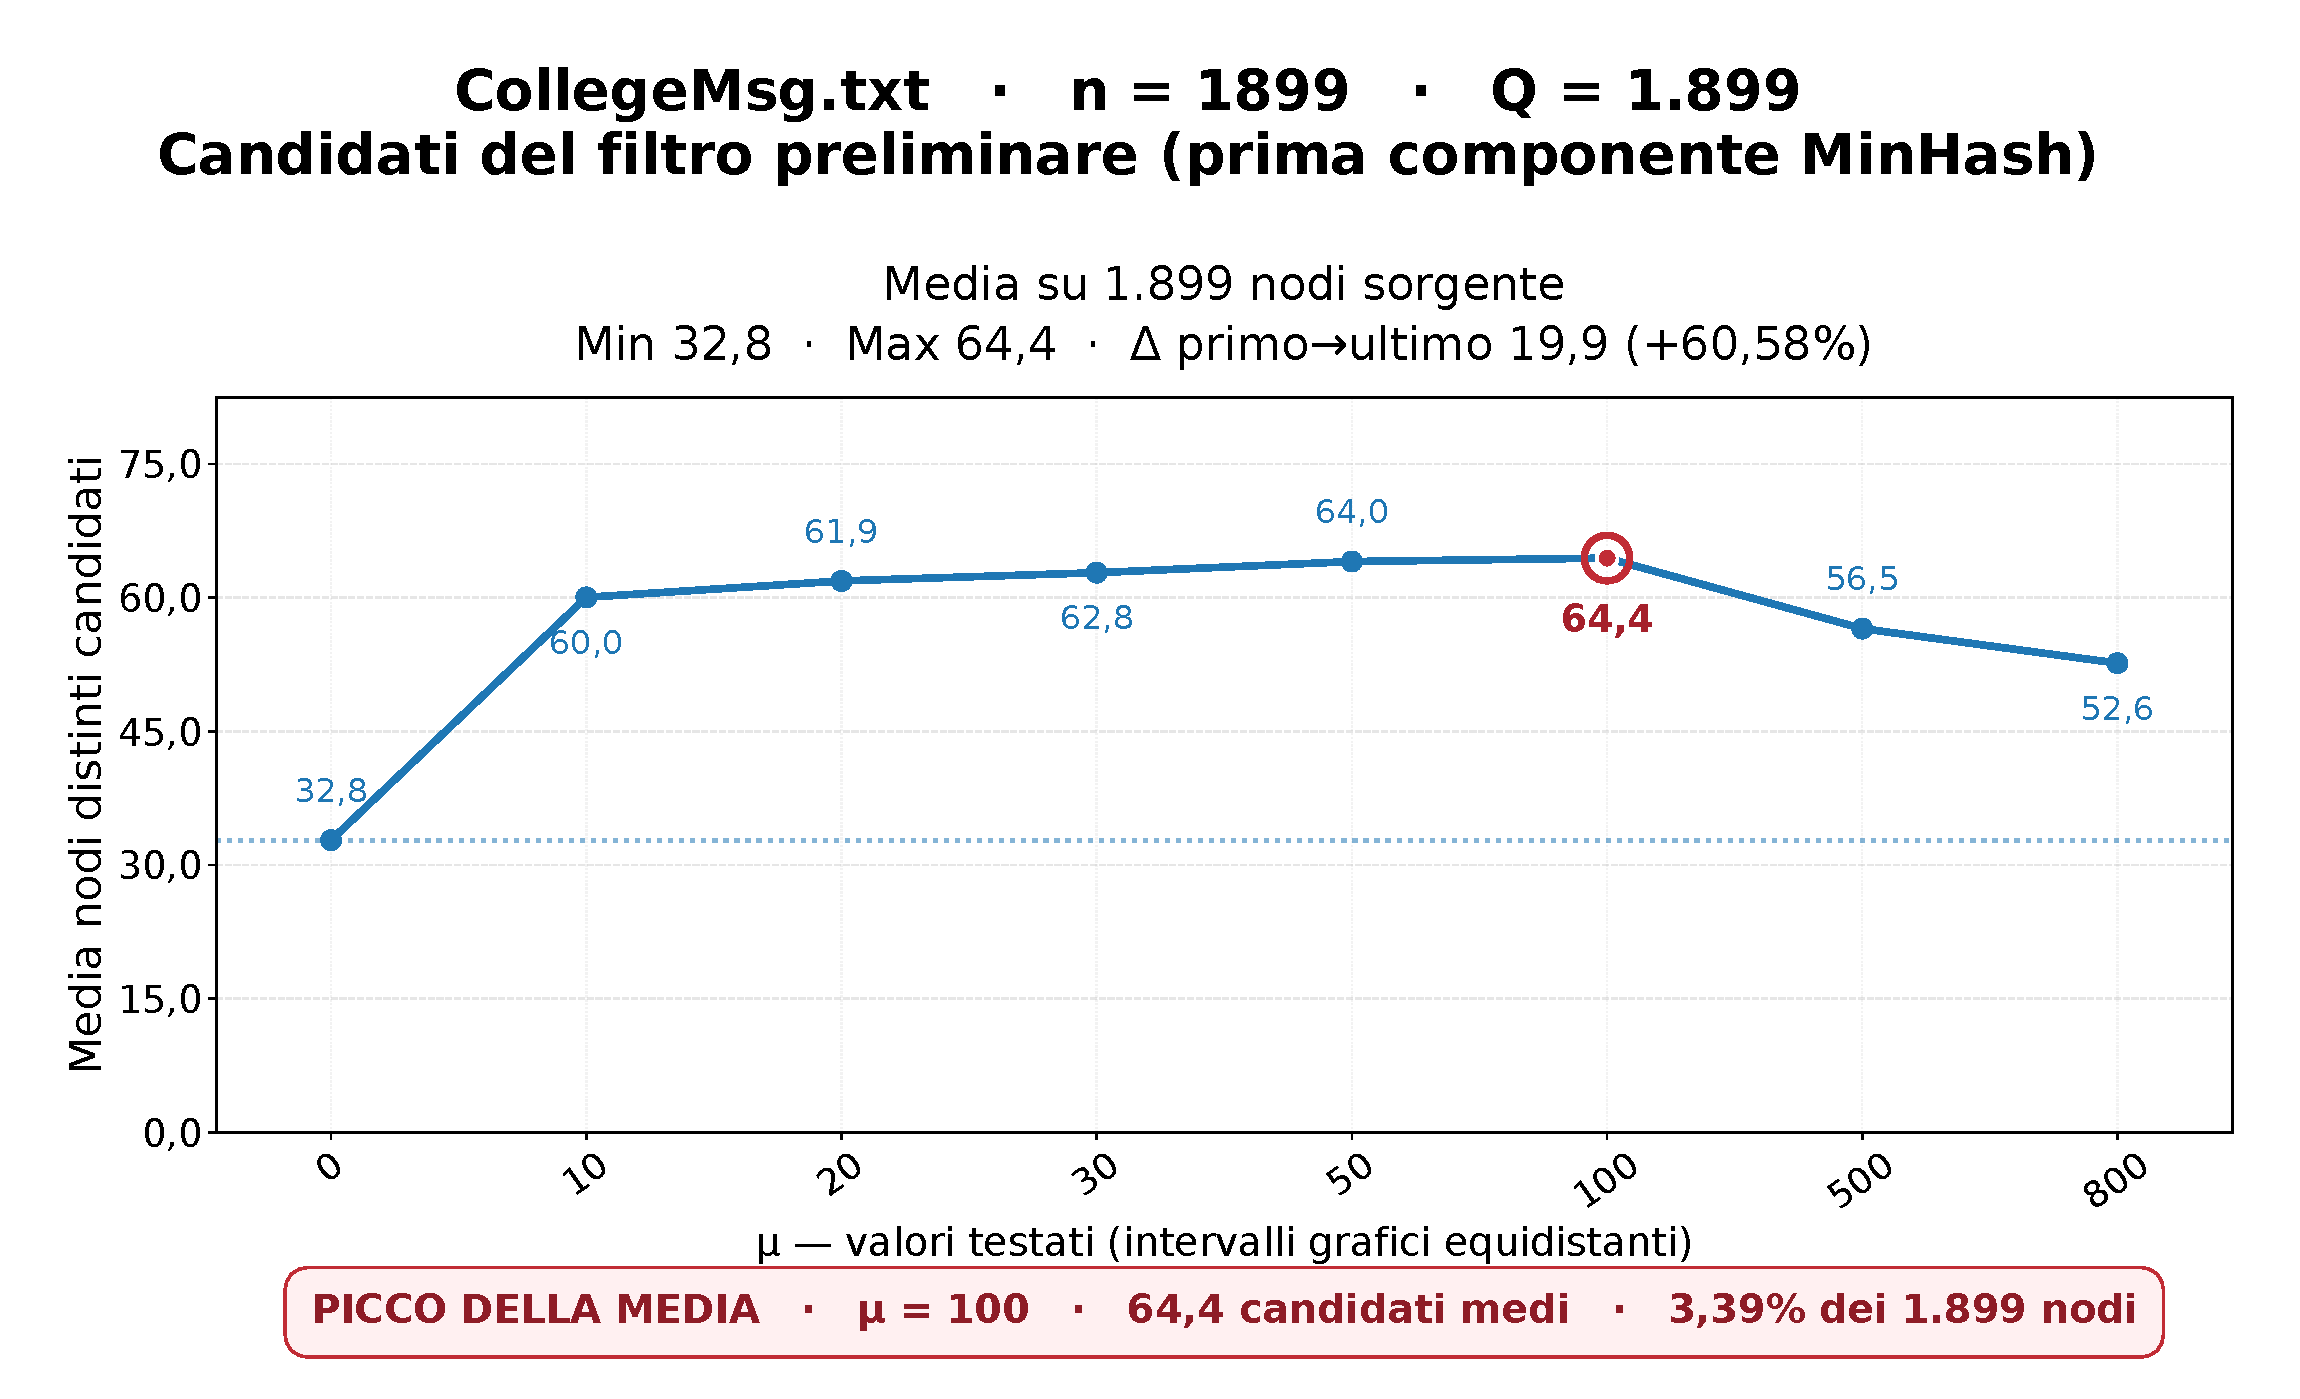
\includegraphics[width=\linewidth,height=4.95cm,keepaspectratio]{figures/CollegeMsg_comparison.pdf}\\[-2pt]
{\small\color{teal}\bfseries 32.8--64.4 candidati su 1\,899 nodi}
\column{.49\textwidth}
\centering
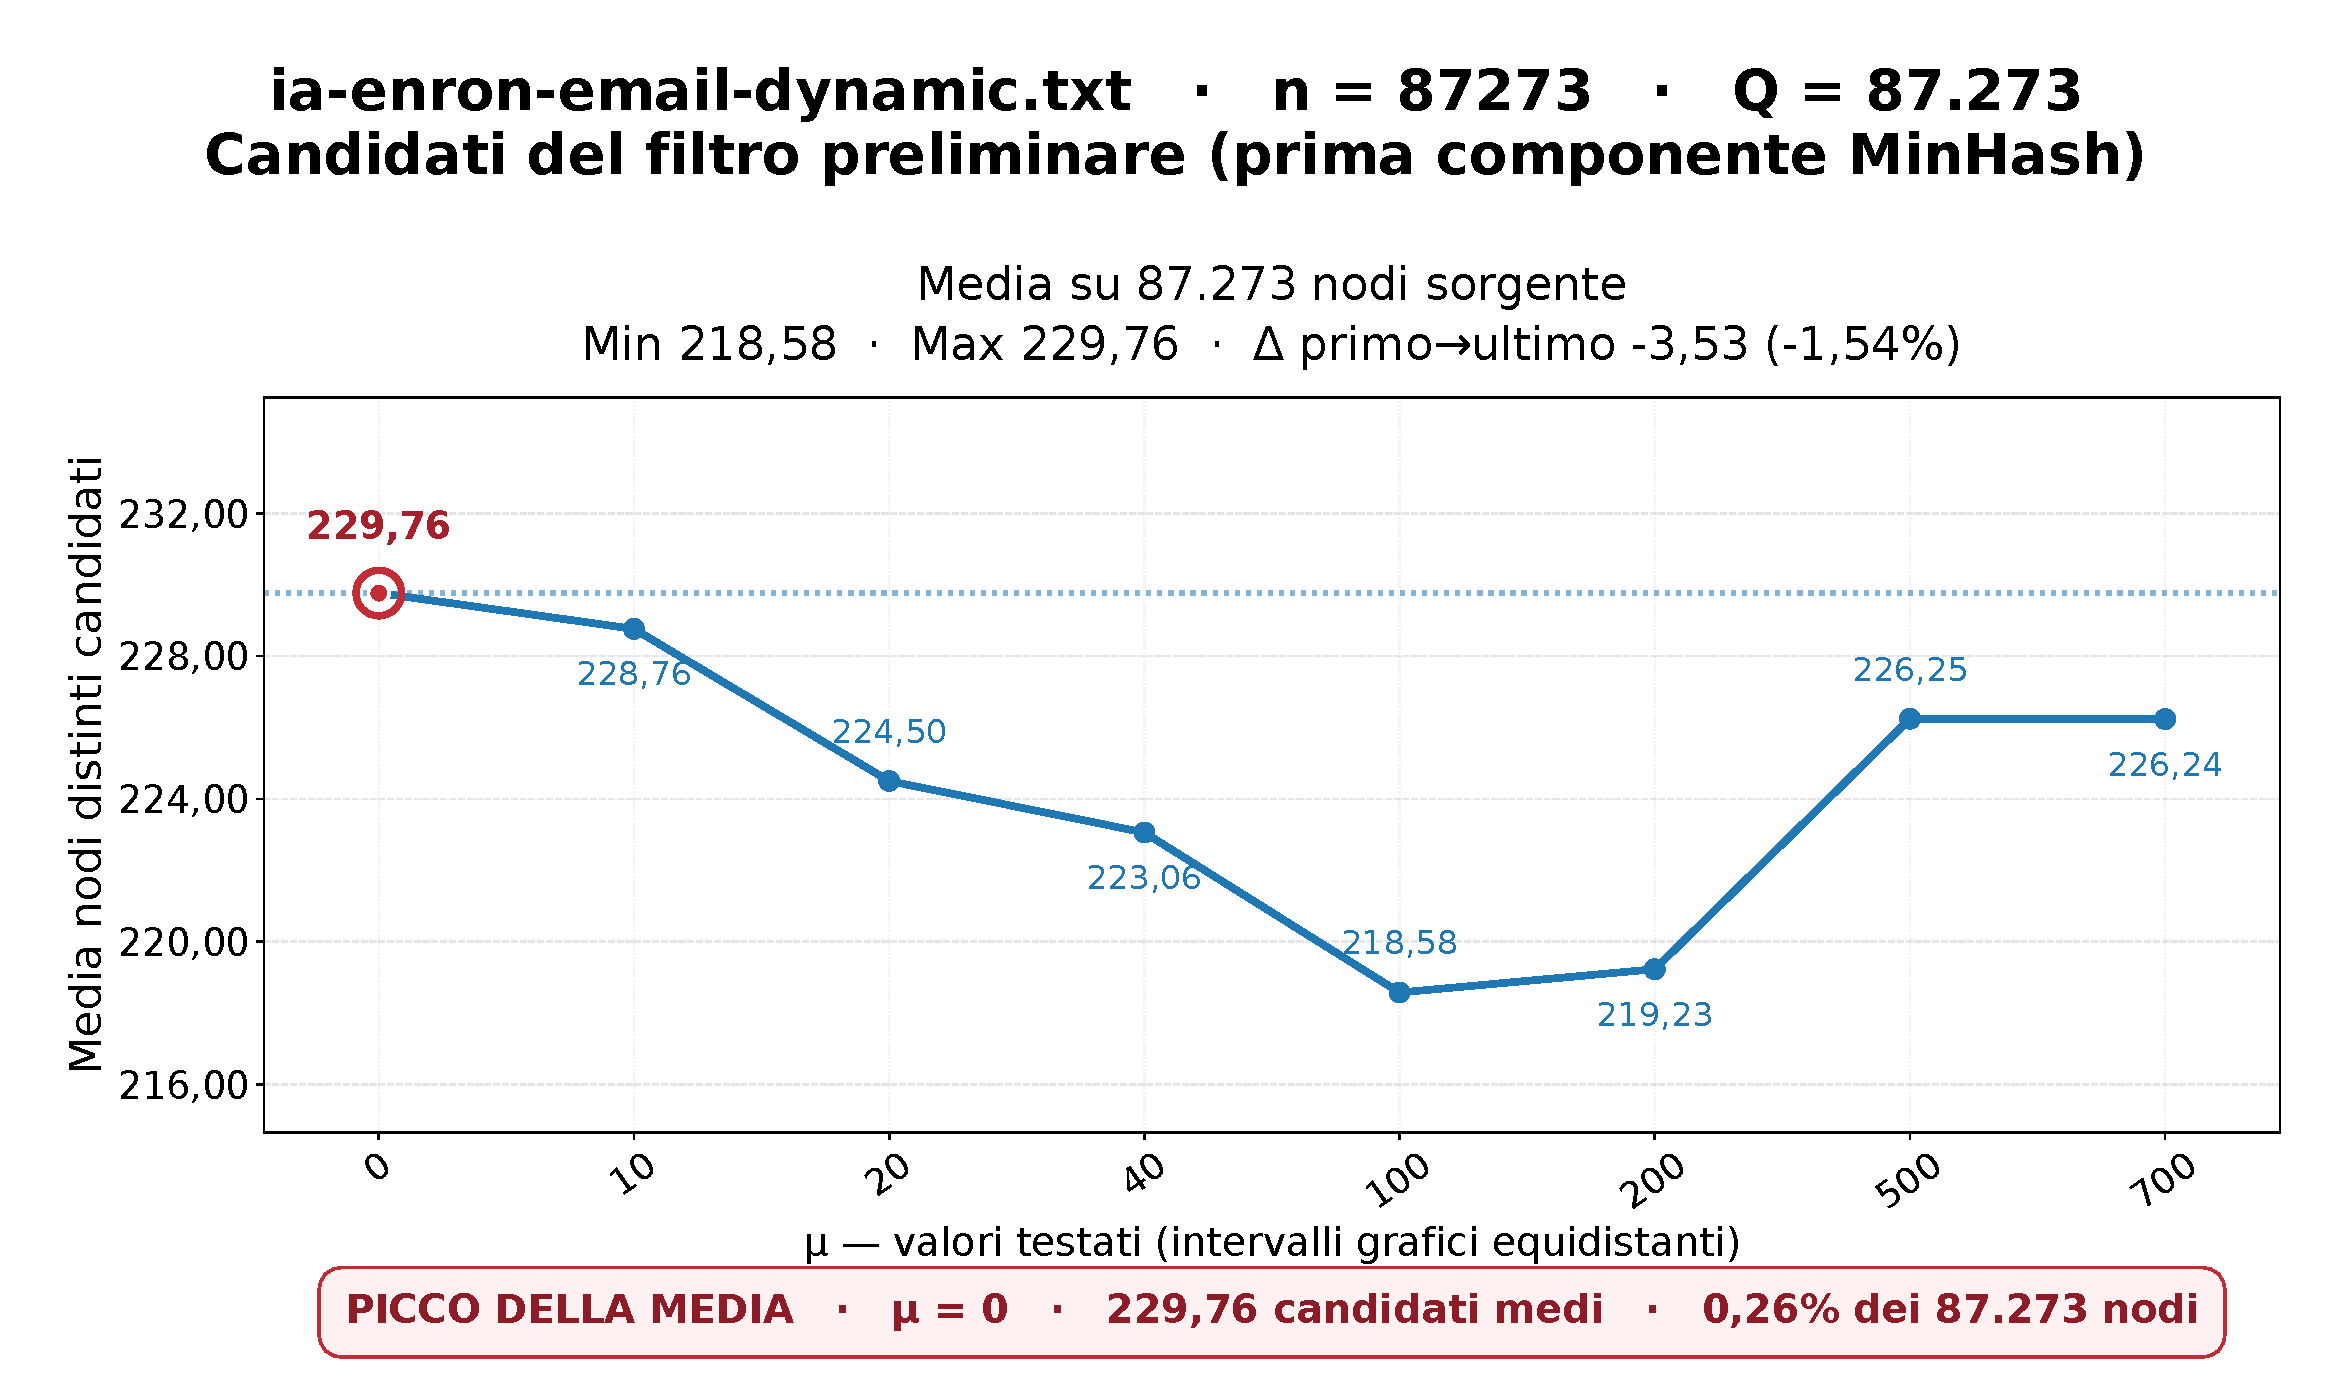
\includegraphics[width=\linewidth,height=4.95cm,keepaspectratio]{figures/ia-enron-email-dynamic_comparison.pdf}\\[-2pt]
{\small\color{teal}\bfseries 218.6--229.8 candidati su 87\,273 nodi}
\end{columns}
\vspace{.20cm}
\smallnote{Esperimento sul solo filtro $C_1(v,\mu)$. Non misura il costo della verifica, la recall o il tempo della query completa. I nodi ripetuti in più finestre si contano una sola volta.}
\end{frame}


\sectslide{04}{Conclusioni e sviluppi futuri}{Contributi, limiti sperimentali e \\direzioni di ricerca}
% 22 — Conclusioni e sviluppi futuri
\section{Conclusioni}
\begin{frame}[t]{Risultati principali e sviluppi futuri}
\vspace{.02cm}
\begin{columns}[T,onlytextwidth]
\column{.50\textwidth}
\centering\panel{5.84cm}{\textbf{Ampiezza fissa}\\[4pt]
\small Indice LSH unificato + pruning + oracolo $\mathcal O$\\[4pt]
{\color{teal}\Large\bfseries $98.2\%$}\\[2pt]\scriptsize finestre scartate su Enron\\[8pt]
}
% {\color{teal}\Large\bfseries $8431\times$}\\[2pt]\scriptsize speedup di query vs BF}
\column{.48\textwidth}
\centering\panel{5.75cm}{\textbf{Ampiezza variabile}\\[4pt]
\small Filtro Euristico \\[4pt]
% {\color{teal}\Large\bfseries $\Theta(T^2)$}$\to${\color{teal}\Large\bfseries $O(T)$}\\[2pt]\scriptsize gruppi di intervalli per nodo\\[8pt]
\small {\color{teal}\Large\bfseries $230 \quad(\approx0.26\%)$}\\[2pt]\scriptsize nodi candidati su Enron.}
\end{columns}
\vspace{.30cm}
\centering
\panel{8.6cm}{\textbf{Prossimi passi}\\[4pt]\small Completare la variante 2,\\studiare altre definizioni di Neighborhood Search\\e modificare i parametri di LSH per ottenere Recall migliori.}
\end{frame}

% 23 — Ringraziamenti
{\setbeamertemplate{footline}{}\begin{frame}[plain]
\begin{tikzpicture}[remember picture,overlay]
  \fill[ink](current page.south west)rectangle(current page.north east);
  \fill[teal!39!ink] ([xshift=9.0cm]current page.south west) circle (4.6cm);
  \foreach \x/\y in {9.8/3.6,11.1/4.9,12.85/4.3,13.3/2.5,10.4/1.6}{\fill[white!75](\x,\y)circle(2.7pt);}
  \foreach \xa/\ya/\xb/\yb in {9.8/3.6/11.1/4.9,11.1/4.9/12.85/4.3,12.85/4.3/13.3/2.5,13.3/2.5/10.4/1.6,10.4/1.6/9.8/3.6}{\draw[white!45,thick](\xa,\ya)--(\xb,\yb);}
  \node[anchor=south west,inner sep=4pt] at ([xshift=-.13cm,yshift=-.38cm]current page.south west)
    {
\includegraphics[width=4.7cm]{figures/TorVergataLogo_no-sfondo.png}};
\end{tikzpicture}
\vspace{2.2cm}
{\color{white}\fontsize{37}{45}\selectfont\bfseries Grazie per l'attenzione!}\par\vspace{.42cm}
{\color{bright}\Large Franco Salvucci}\par\vspace{.19cm}
{\color{white!80}\small Il Problema del Neighborhood Search su Grafi Temporali}
\end{frame}}

% 19 — T^2 intervalli raggruppati in T rettangoli
\begin{frame}[t]{Dagli intervalli ai rettangoli geometrici}
\vspace{-.14cm}
\begin{columns}[T,onlytextwidth]
\column{.52\textwidth}
\centering
\begin{tikzpicture}[x=.83cm,y=.68cm]
  % Bounding box fissa su tutti e quattro gli overlay.
  \path[use as bounding box] (.10,-.42) rectangle (6.65,6.23);
  \only<1>{
    % Cinque intervalli di esempio lungo un orizzonte di T istanti.
    \draw[-{Stealth[length=2.4mm]},thick,muted]
      (.68,1.0)--(6.25,1.0) node[right,font=\small]{$t$};
    \foreach \x/\lab in {1.10/1,2.15/2,3.20/3,4.25/4,5.30/5}{
      \draw[rulegray,thick](\x,.85)--(\x,1.16);
      \node[font=\scriptsize,text=muted] at (\x,.52) {$t_{\lab}$};
    }
    \node[font=\small\bfseries,text=teal] at (3.40,5.59)
      {Intervalli temporali di esempio};
    \foreach \ys/\xa/\xb/\lab/\col in {
      4.84/1.10/3.20/I_1/teal,
      4.04/2.15/4.25/I_2/gold,
      3.24/3.20/5.30/I_3/teal,
      2.44/1.10/4.25/I_4/gold,
      1.64/2.15/5.30/I_5/teal}{
      \draw[\col,line width=4pt,line cap=round](\xa,\ys)--(\xb,\ys);
      \fill[\col](\xa,\ys) circle (3.2pt);
      \fill[\col](\xb,\ys) circle (3.2pt);
      \node[font=\scriptsize\bfseries,text=\col,anchor=east] at (.90,\ys)
        {$\lab$};
    }
    \node[font=\scriptsize,text=muted,align=center] at (3.38,-.02)
      {Ogni intervallo è definito da due estremi.};
  }
  \visible<2->{
    % Gli estremi diventano coordinate nel piano T x T.
    \foreach \x in {1.10,2.15,3.20,4.25,5.30}{
      \draw[rulegray!58,line width=.35pt](\x,.72)--(\x,5.72);
      \draw[rulegray!58,line width=.35pt](.70,\x)--(5.85,\x);
    }
    \draw[-{Stealth},thick,muted](.5,.52)--(6.4,.52)
      node[below,font=\small]{$\alpha$};
    \draw[-{Stealth},thick,muted](.5,.52)--(.5,6.1)
      node[left,font=\small]{$\beta$};
  }
  \visible<3->{
    % Ogni punto dell'esempio cade in un rettangolo della sua classe MinHash.
    \fill[ice,opacity=.85] (.90,2.92) rectangle (2.42,4.63);
    \draw[teal,thick] (.90,2.92) rectangle (2.42,4.63);
    \fill[gold!16,opacity=.85] (1.93,5.01) rectangle (3.47,5.61);
    \draw[gold,thick] (1.93,5.01) rectangle (3.47,5.61);
    \node[font=\tiny\bfseries,text=teal!80!black] at (1.67,3.70) {$h_1=a$};
    \node[font=\tiny\bfseries,text=gold!80!black] at (2.74,5.42) {$h_1=b$};
  }
  \visible<2->{
    % Punti corrispondenti, nell'ordine, agli stessi intervalli del primo overlay.
    \foreach \x/\y in {1.10/3.20,2.15/4.25,3.20/5.30,1.10/4.25,2.15/5.30}{
      \fill[ink] (\x,\y) circle (3.0pt);
      \draw[white,line width=.50pt] (\x,\y) circle (3.0pt);
    }
  }
  \only<2>{
    \node[font=\tiny,text=ink,anchor=west] at (1.20,3.10) {$I_1$};
    \node[font=\tiny,text=ink,anchor=west] at (2.25,4.15) {$I_2$};
    \node[font=\tiny,text=ink,anchor=west] at (3.30,5.20) {$I_3$};
    \node[font=\tiny,text=ink,anchor=east] at (1.00,4.18) {$I_4$};
    \node[font=\tiny,text=ink,anchor=east] at (2.05,5.22) {$I_5$};
  }
  \visible<4->{
    % D_mu per mu=2 attraversa esattamente i punti I_1, I_2 e I_3.
    \draw[coral,line width=1.8pt] (.82,2.92)--(3.54,5.64);
    \node[font=\small,text=coral] at (4.25,2.30)
      {$D_\mu:\ \beta=\alpha+\mu$};
  }
  \only<2>{\node[font=\scriptsize,text=muted,align=center] at (2.97,.02)
      {Intervallo $[\alpha,\beta]$ $\longmapsto$ punto $(\alpha,\beta)$};}
  \only<3>{\node[font=\scriptsize,text=muted,align=center] at (2.97,.02)
      {Stesso valore MinHash: stesso rettangolo.};}
  \only<4->{\node[font=\scriptsize,text=muted,align=center] at (2.97,.02)
      {La retta $D_\mu$ seleziona le finestre di ampiezza $\mu$.};}
\end{tikzpicture}
\column{.46\textwidth}
\vspace{.34cm}
\uncover<3->{\panel{5.37cm}{\textbf{Idea geometrica}\\[8pt]
\small Il primo MinHash resta costante su famiglie di intervalli rappresentabili con rettangoli.\\[7pt]
$\Theta(T^2)$ intervalli $\longrightarrow$ al più $T$ rettangoli per nodo.}}
\vspace{.22cm}
\uncover<4->{\panel{5.37cm}{\textbf{Query di ampiezza $\mu$}\\[8pt]
\small Si cercano rettangoli con la stessa etichetta che intersecano la retta $D_\mu$.}}
\end{columns}
% La complessità del Range Tree è mostrata nella slide successiva.
\end{frame}

% 20 — Bound teorici variante 2
\begin{frame}[t]{Costi teorici del filtro geometrico}
\vspace{.06cm}
\begin{center}\small $M$: coppie riportate dal filtro.\end{center}
\vspace{.27cm}
\begin{columns}[T,onlytextwidth]
\column{.33\textwidth}
\centering\panel{4.08cm}{\textbf{Building time}\\[14pt]
$\displaystyle O\!\left(|\mathcal E|+nT\log^3nT\right)$\\[12pt]}
\column{.33\textwidth}
\centering\panel{4.08cm}{\textbf{Spazio}\\[14pt]
$\displaystyle O\!\left(nT\log^3nT\right)$\\[12pt]}
\column{.33\textwidth}
\centering\panel{4.08cm}{\textbf{Identificare i candidati}\\[14pt]
$\displaystyle O\!\left(T\log^3nT+M\right)$\\[12pt]}
\end{columns}
\vspace{.34cm}
\begin{center}\chip{La verifica finale con le signature complete è esclusa da questi bound.}\end{center}
\vspace{.17cm}
\smallnote{Non esiste un bound non banale sul numero di candidati $M$: la selettività del filtro dipende dai dati e dalla permutazione MinHash.}
\end{frame}

\end{document}
